As introduced in \cref{Introduction}, this thesis explores the generation of counterfactual explanations (CEs) in image-based autonomous driving scenarios using deep generative models and post-hoc interpretability techniques. The corresponding implementations are detailed in \cref{Methodology}.

This chapter presents the evaluation strategy and experimental findings, structured according to the central research questions (RQs). For each RQ, the evaluation criteria are outlined and later expanded in dedicated result sections.

\textbf{RQ1:} \textit{How can deep generative models be implemented to effectively encode and reconstruct images of high-dimensional driving scenes for interpretable and compact representation learning in autonomous driving systems?}

\vspace{-1em}

\paragraph{Evaluation:}The VAE is evaluated on two primary fronts: (i) the fidelity of reconstructed images, and (ii) the semantic usefulness of the latent representations for downstream classification. To this end, multiple classifiers—including MLP, SVM, KNN, Logistic Regression, and Random Forest—are trained on the latent vectors extracted by the encoder. Classification performance is assessed for both binary (GO vs. STOP) and multi-class (GO, STOP, LEFT, RIGHT) tasks. Evaluation metrics include reconstruction loss, pixel accuracy, PSNR, classification accuracy, precision, recall, and F1-score.
    
\vspace{1em}

\textbf{RQ1:} \textit{How can loss function modifications in Variational Autoencoders (VAEs) optimize image reconstruction quality in autonomous driving tasks?} 

\vspace{-1em}

\paragraph{Evaluation:}Compare the image quality Structural Similarity Index (SSIM) and Peak Signal-to-Noise Ratio (PSNR) and classification metrics (accuracy, F1) between a standard VAE and one using modified loss functions. This will include both quantitative analysis and qualitative visualizations of reconstructed images.

\vspace{1em}
    
\textbf{RQ3:} \textit{How do different masking techniques impact the effectiveness and efficiency of counterfactual explanation generation, in terms of coverage, computational cost, method overlap, and failure rate? (See \cref{Methodology} for details on the techniques investigated.)}

\vspace{-1em}

\paragraph{Evaluation:} To assess each method, the following criteria are measured during CE generation:
    \begin{itemize}
        \item \textbf{Coverage:} Proportion of total inputs for which valid counterfactual explanations are successfully generated.
        \item \textbf{Computational Cost:} Average time taken per sample for each method.
        \item \textbf{Failure Rate:} Percentage of inputs for which no counterfactual explanations was found.
        \item \textbf{Method Overlap:} Instances where multiple masking techniques generate the same counterfactual explanations.
        \item \textbf{Visual Quality:} SSIM, and PSNR metrics between original and reconstructed images.
    \end{itemize}

    All masking methods are applied to the same dataset split, using identical model checkpoints for the VAE and classifier. This ensures fair and consistent comparisons across metrics.

\vspace{1em}

\textbf{RQ4:} \textit{ Which counterfactual explanation method is preferred by users when selecting among generated explanations of the same original image? What factors influence user preference? (See \cref{Methodology} for details on the methods compared.)}

\vspace{-1em}

\paragraph{Evaluation:} Evaluation is based on aggregated user responses:
    \begin{itemize}
        \item \textbf{Preference Distribution:} Percentage of total selections made per CE method.
        \item \textbf{Attribute Ratings:} Average scores for interpretability, plausibility, and coherence across methods.
        \item \textbf{Qualitative Feedback:} Comments collected through optional text fields to gain insights into user reasoning.
    \end{itemize}

This dual analysis enables the identification of methods that are not only algorithmically effective but also intuitively meaningful to end users critical for real-world deployment of interpretable AI in autonomous systems.
    


Each of the following sections restates the respective RQ, evaluates the implemented methods against that question, and presents results along with a discussion of key findings.


\section{Evaluation of Variational Autoencoder (RQ1, RQ2)} \label{sec:vae_evaluation}

The Variational Autoencoder (VAE) forms the backbone of this thesis. It serves dual purposes: (i) as a deep generative model that enables the reconstruction and manipulation of high-dimensional driving scene images, and (ii) as a representation learning tool to generate low-dimensional, semantically meaningful latent vectors suitable for downstream driving action classification. The quality of both image reconstruction and latent encoding is crucial for the success of counterfactual generation. Therefore, evaluating the VAE both quantitatively and qualitatively is a vital first step.

To ensure robustness, various architectural configurations and hyperparameter settings were explored, including latent dimensionality, convolutional depth, and KL divergence annealing schedules. One major focus was the choice of reconstruction loss function, which has a significant effect on the quality of output and the stability of training. Two variants were trained. One using traditional Mean Squared Error (MSE) and the other using Log-Cosh, a smoother, outlier-robust alternative motivated by prior work by Chen et al.,~\cite{chen2019log}. This section presents the training dynamics, comparative results between the two losses, and the final analysis of latent space quality.

\subsection{Training Performance and Loss Analysis} \label{subsubsec:vae_training_loss}

Two VAE variants were trained for 200 epochs each, differing only in their reconstruction loss: Mean Squared Error (MSE) and Log-Cosh. Throughout training, we monitored several key metrics:

\begin{itemize}
    \item \textbf{Total Loss:} Sum of reconstruction and KL divergence losses.
    \item \textbf{Reconstruction Loss:} Measures pixel-wise reconstruction error.
    \item \textbf{KL Divergence:} Reflects the alignment of the latent space distribution with a unit Gaussian prior.
    \item \textbf{Validation Pixel Accuracy:} Measures how accurately the reconstructed image matches the original at pixel level.
    \item \textbf{PSNR (Peak Signal-to-Noise Ratio):} Evaluates perceptual reconstruction quality.
\end{itemize}

\textbf{Log-Cosh Variant (Figures \ref{fig:logcosh_kl_loss} to \ref{fig:logcosh_psnr})}

\begin{itemize}
    \item \textbf{KL Divergence:} As shown in Figure~\ref{fig:logcosh_kl_loss}, KL loss rapidly decreased in the early epochs and gradually stabilized, indicating that the annealing schedule successfully encouraged disentangled latent features.
    \item \textbf{Reconstruction \& Total Loss:} Both training and validation losses (Figures~\ref{fig:logcosh_recon_loss} and \ref{fig:logcosh_total_loss}) show a smooth, monotonic decrease, suggesting stable convergence.
    \item \textbf{Pixel Accuracy \& PSNR:} Validation pixel accuracy steadily increased, reaching 0.97 (Figure~\ref{fig:logcosh_val_acc}), while PSNR improved consistently to 31.4 dB (Figure~\ref{fig:logcosh_psnr}).
\end{itemize}

A qualitative comparison of the reconstructed image at epoch 200 (Figure~\ref{fig:logcosh_epoch200}) shows that the VAE preserves semantic structure and texture remarkably well.

\begin{figure}[htbp]
    \centering
    \begin{subfigure}[b]{0.45\textwidth}
        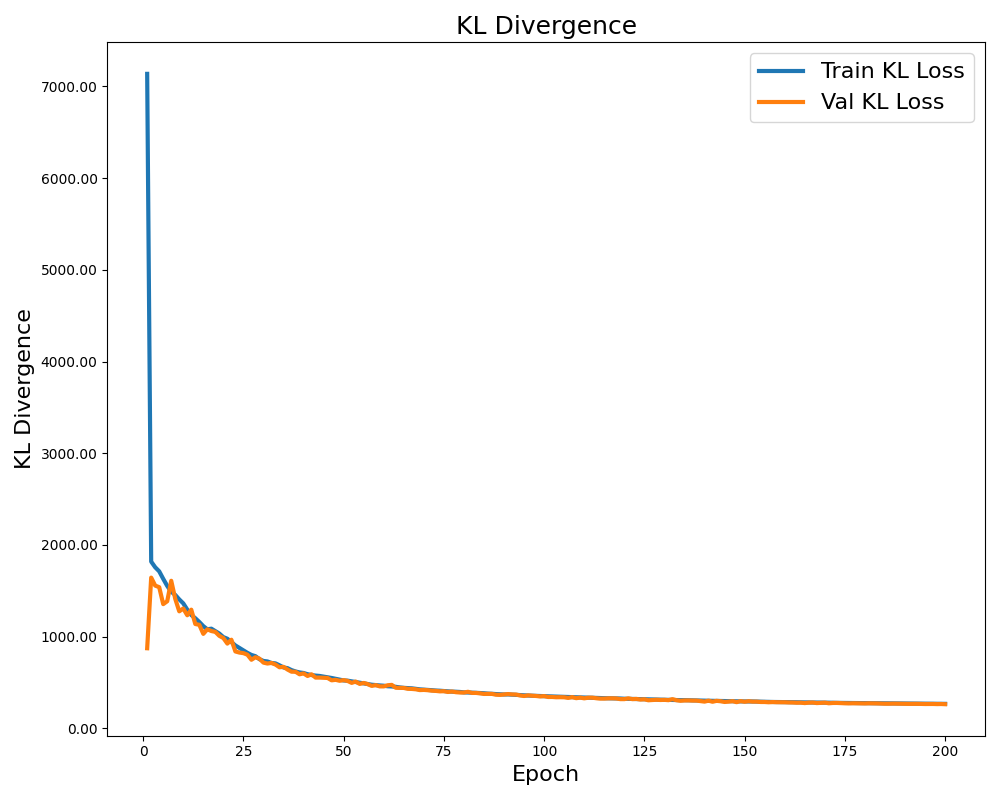
\includegraphics[width=\textwidth]{img/vae_results/200_epochs_128_ls_logcosh/logcosh_kl_loss.png}
        \caption{KL divergence over epochs for VAE trained with Log-Cosh loss.}
        \label{fig:logcosh_kl_loss}
    \end{subfigure}
    \hfill
    \begin{subfigure}[b]{0.45\textwidth}
        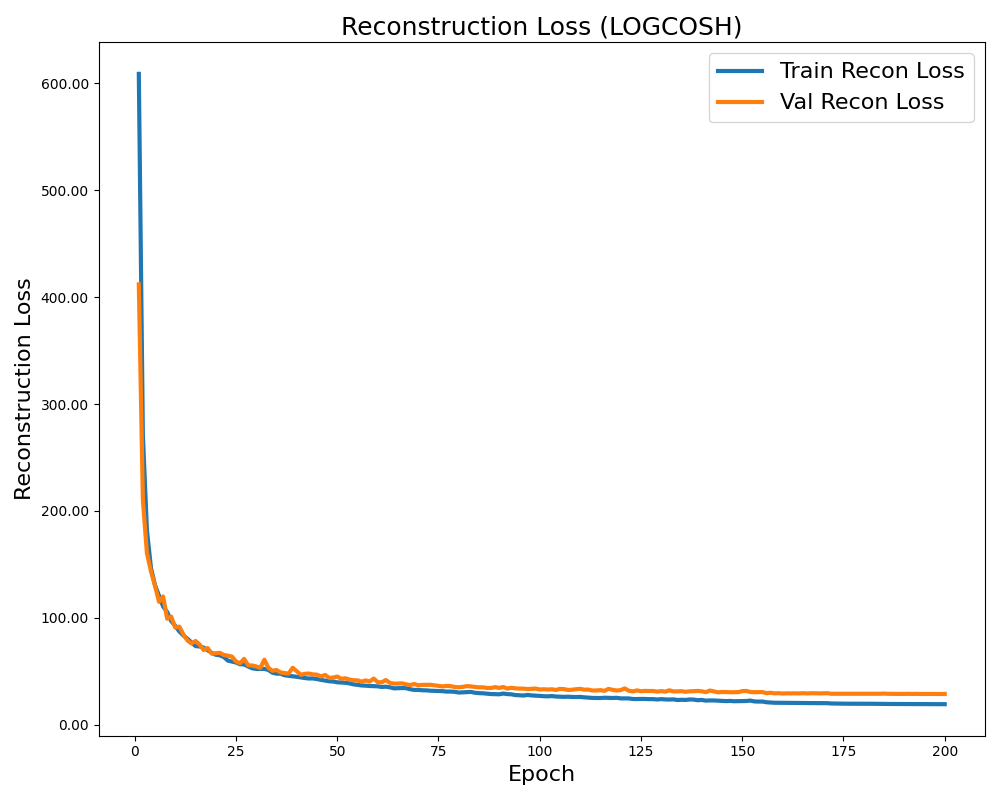
\includegraphics[width=\textwidth]{img/vae_results/200_epochs_128_ls_logcosh/logcosh_recon_loss.png}
        \caption{Reconstruction loss over epochs (Log-Cosh).}
        \label{fig:logcosh_recon_loss}
    \end{subfigure}
    
    \begin{subfigure}[b]{0.45\textwidth}
        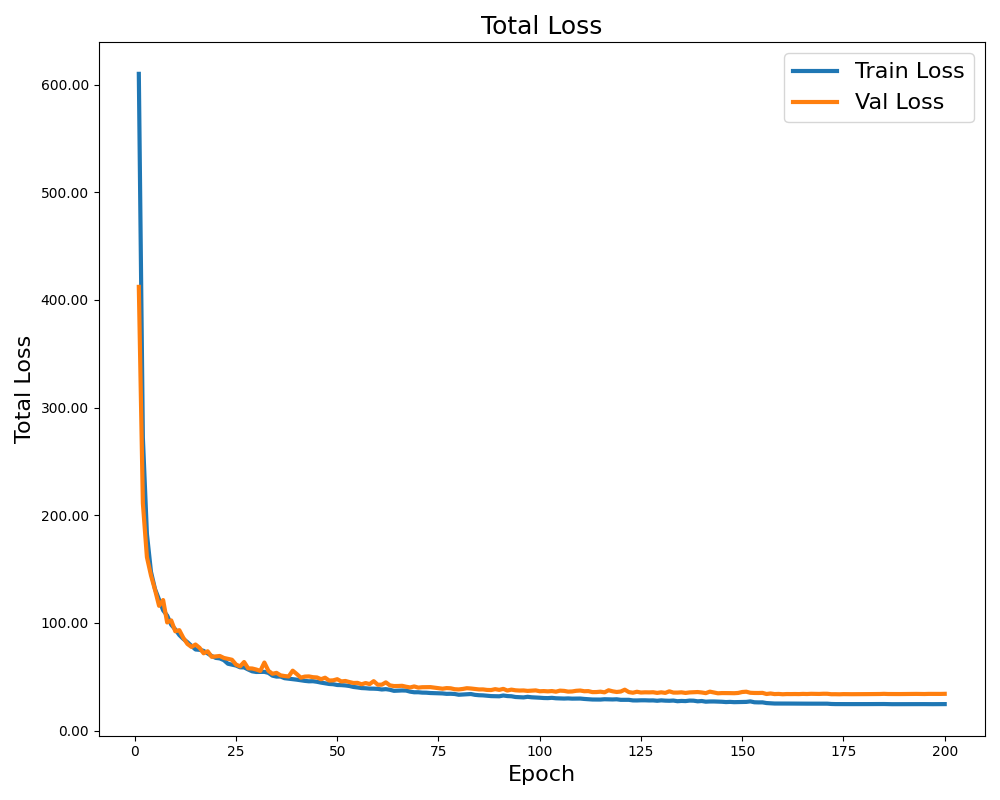
\includegraphics[width=\textwidth]{img/vae_results/200_epochs_128_ls_logcosh/logcosh_total_loss.png}
        \caption{Total loss over epochs (Log-Cosh).}
        \label{fig:logcosh_total_loss}
    \end{subfigure}
    \hfill
    \begin{subfigure}[b]{0.45\textwidth}
        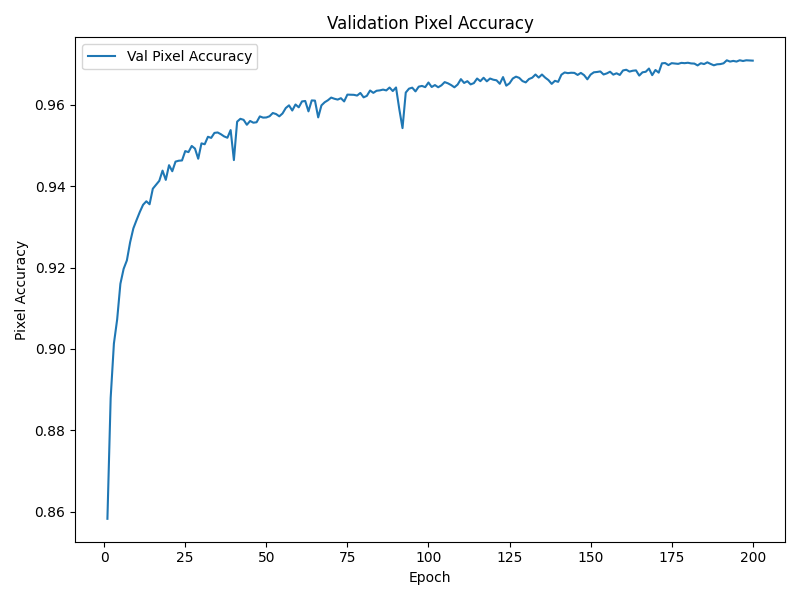
\includegraphics[width=\textwidth]{img/vae_results/200_epochs_128_ls_logcosh/logcosh_val_accuracy.png}
        \caption{Validation pixel accuracy across epochs (Log-Cosh).}
        \label{fig:logcosh_val_acc}
    \end{subfigure}
    
    \begin{subfigure}[b]{0.45\textwidth}
        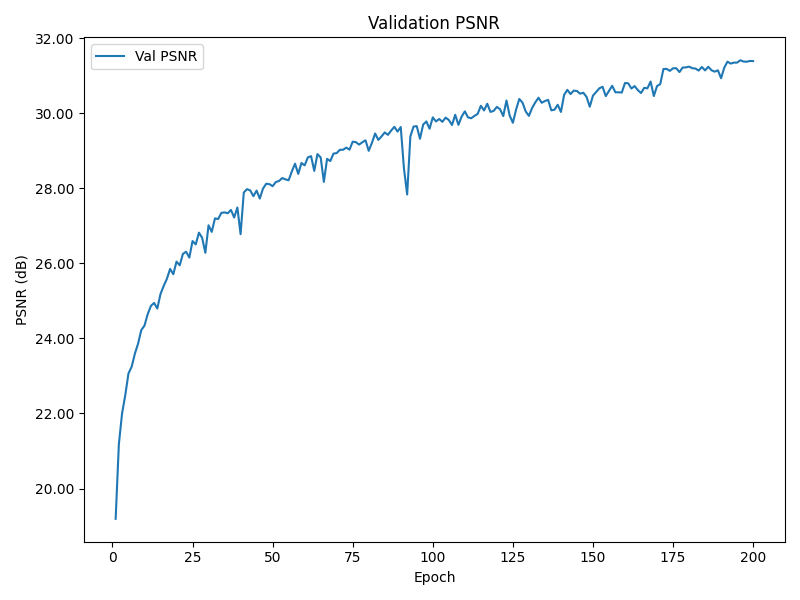
\includegraphics[width=\textwidth]{img/vae_results/200_epochs_128_ls_logcosh/logcosh_val_psnr.png}
        \caption{Validation PSNR trajectory for Log-Cosh model.}
        \label{fig:logcosh_psnr}
    \end{subfigure}
    \hfill
    \begin{subfigure}[b]{0.45\textwidth}
        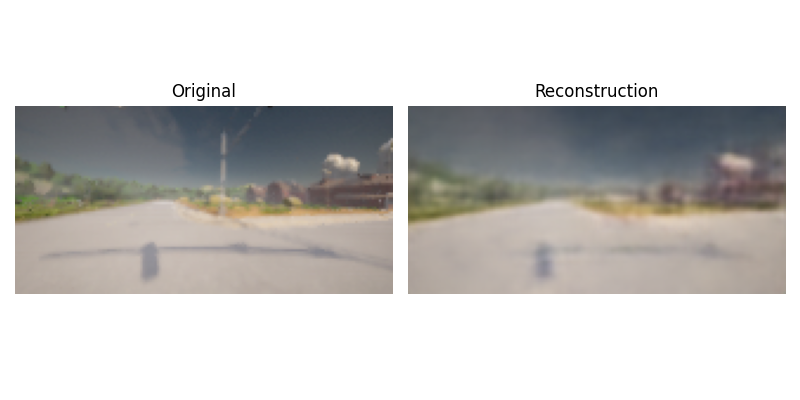
\includegraphics[width=\textwidth]{img/vae_results/200_epochs_128_ls_logcosh/reconstructions/epoch_200.png}
        \caption{Original vs. Reconstructed image at epoch 200 (Log-Cosh).}
        \label{fig:logcosh_epoch200}
    \end{subfigure}
    
    \caption{Training Performance and Loss Analysis for Log-Cosh Variant: Detailed analysis of the VAE's performance using the Log-Cosh loss function, highlighting key metrics and qualitative results.}
    \label{fig:logcosh_analysis}
\end{figure}




\subsection{Training Comparison with MSE Loss} \label{subsubsec:vae_mse_loss}

The training curves for the MSE-based VAE show similar convergence trends but at a consistently higher loss level across all metrics:

\begin{itemize}
    \item \textbf{Total and Reconstruction Loss:} Figures~\ref{fig:mse_total_loss} and \ref{fig:mse_recon_loss} indicate slower and less stable convergence compared to Log-Cosh.
    \item \textbf{Pixel Accuracy \& PSNR:} Slightly lower final accuracy (~0.969) and PSNR (30.99 dB), as seen in Figures~\ref{fig:mse_val_acc} and \ref{fig:mse_val_psnr}.
\end{itemize}

Qualitative Comparison: Figure~\ref{fig:mse_epoch200} shows noticeable blur and loss of fine structure in the reconstructions compared to Log-Cosh.

\begin{figure}[htbp]
    \centering
    \begin{subfigure}[b]{0.45\textwidth}
        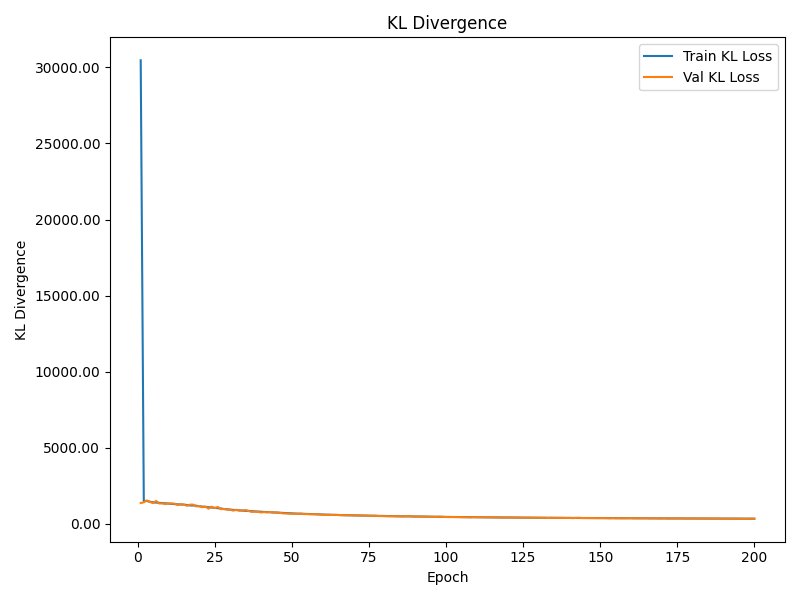
\includegraphics[width=\textwidth]{img/vae_results/200_epochs_128_ls_mse/mse_kl_loss.png}
        \caption{KL divergence over epochs for VAE trained with MSE loss.}
        \label{fig:mse_kl_loss}
    \end{subfigure}
    \hfill
    \begin{subfigure}[b]{0.45\textwidth}
        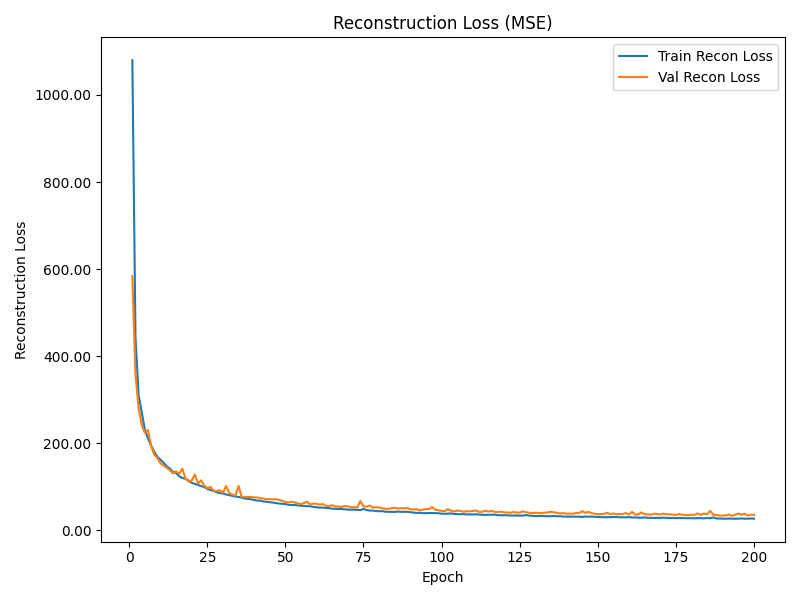
\includegraphics[width=\textwidth]{img/vae_results/200_epochs_128_ls_mse/mse_recon_loss.png}
        \caption{Reconstruction loss over epochs (MSE).}
        \label{fig:mse_recon_loss}
    \end{subfigure}
    
    \begin{subfigure}[b]{0.45\textwidth}
        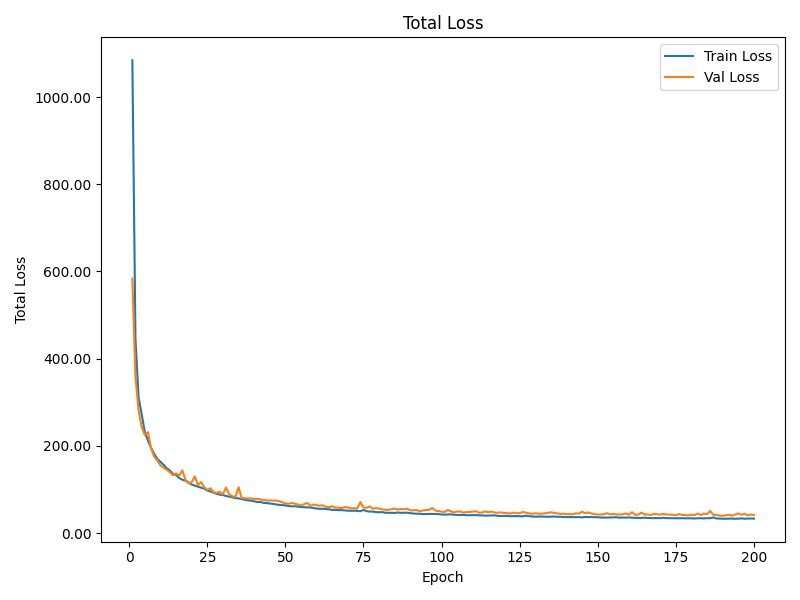
\includegraphics[width=\textwidth]{img/vae_results/200_epochs_128_ls_mse/mse_total_loss.png}
        \caption{Total loss over epochs (MSE).}
        \label{fig:mse_total_loss}
    \end{subfigure}
    \hfill
    \begin{subfigure}[b]{0.45\textwidth}
        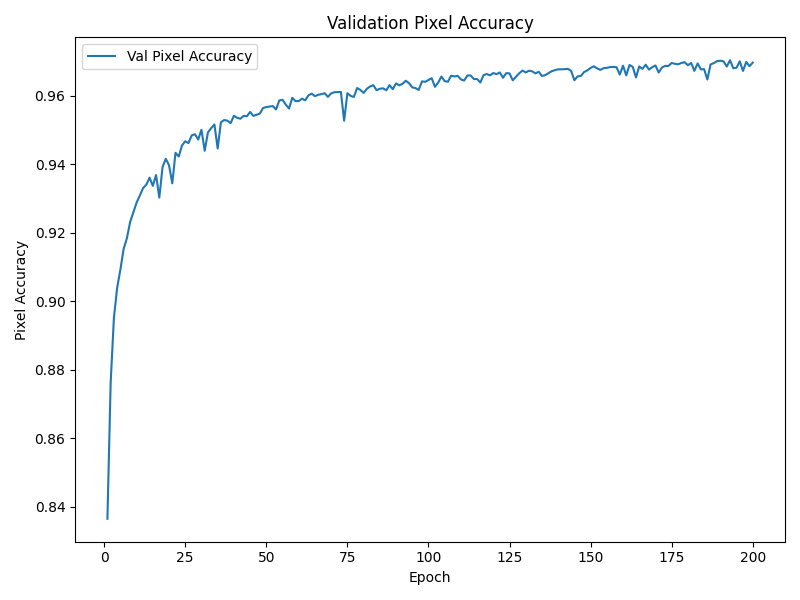
\includegraphics[width=\textwidth]{img/vae_results/200_epochs_128_ls_mse/mse_val_accuracy.png}
        \caption{Validation pixel accuracy across epochs (MSE).}
        \label{fig:mse_val_acc}
    \end{subfigure}
    
    \begin{subfigure}[b]{0.45\textwidth}
        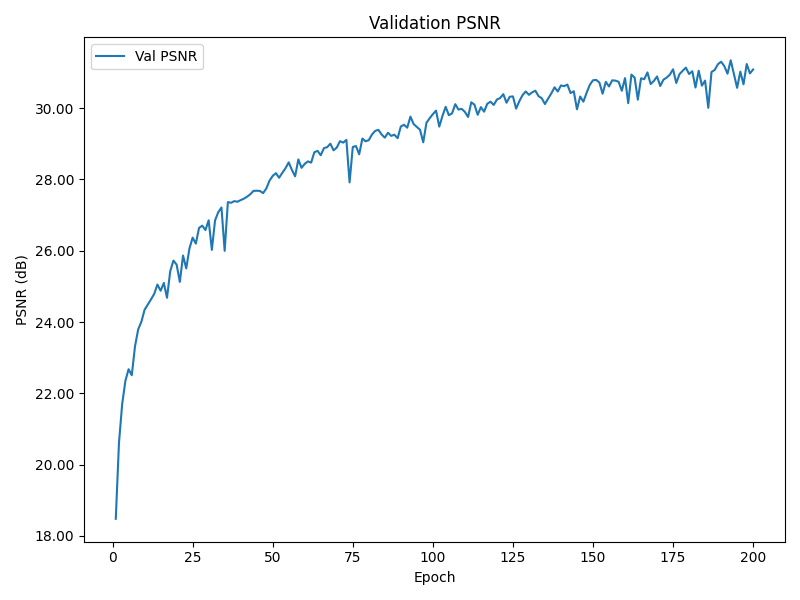
\includegraphics[width=\textwidth]{img/vae_results/200_epochs_128_ls_mse/mse_val_psnr.png}
        \caption{Validation PSNR trajectory for MSE model.}
        \label{fig:mse_val_psnr}
    \end{subfigure}
    \hfill
    \begin{subfigure}[b]{0.45\textwidth}
        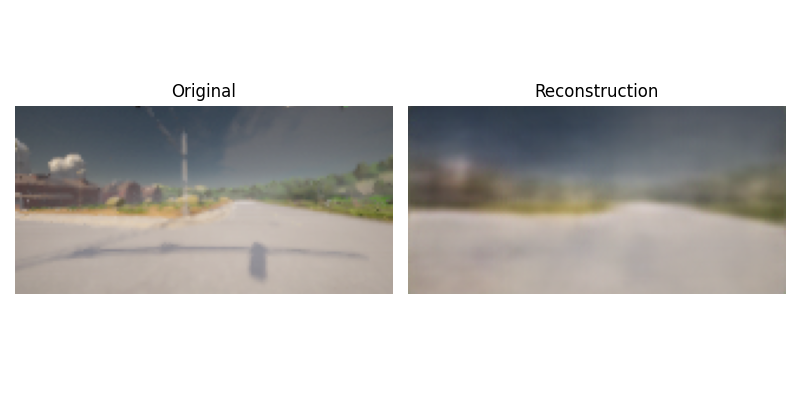
\includegraphics[width=\textwidth]{img/vae_results/200_epochs_128_ls_mse/reconstructions/epoch_200.png}
        \caption{Original vs. Reconstructed image at epoch 200 (MSE).}
        \label{fig:mse_epoch200}
    \end{subfigure}
    
    \caption{Training Performance and Loss Analysis for MSE Variant: A comparison of the VAE's performance using MSE loss, highlighting differences in convergence and reconstruction quality compared to Log-Cosh.}
    \label{fig:mse_analysis}
\end{figure}










\subsection{Quantitative Comparison of Loss Functions (RQ2 Answered)} \label{subsec:vae_quant_comparison}
To assess the performance of the Variational Autoencoder (VAE), both the Log-Cosh and Mean Squared Error (MSE) loss functions were evaluated across several metrics, namely Total Loss, Reconstruction Loss, KL Divergence, Validation Pixel Accuracy, Peak Signal-to-Noise Ratio (PSNR). 

Table~\ref{tab:loss_comparison} presents average values over the final 5 epochs for both variants:

\begin{table}[h]
    \centering
    \begin{tabular}{lcc}
        \toprule
        \textbf{Metric} & \textbf{Log-Cosh (Avg)} & \textbf{MSE (Avg)} \\
        \midrule
        Validation Total Loss & 21.82 & 42.35 \\
        Validation Reconstruction Loss & 16.49 & 35.84 \\
        Validation KL Divergence & 268.72 & 327.90 \\
        Validation Pixel Accuracy & 0.971 & 0.969 \\
        Validation PSNR (dB) & 31.39 & 30.99 \\
        \bottomrule
    \end{tabular}
    \caption{Comparison of validation metrics for VAE variants (Final 5 Epoch Average)}
    \label{tab:loss_comparison}
\end{table}

Additionally, Figures~\ref{fig:val_loss_comparison} and \ref{fig:val_psnr_comparison} provide a side-by-side comparison of Validation Loss and PSNR over all epochs.


\begin{figure}[h]
    \centering
    \begin{subfigure}[b]{0.49\textwidth}
        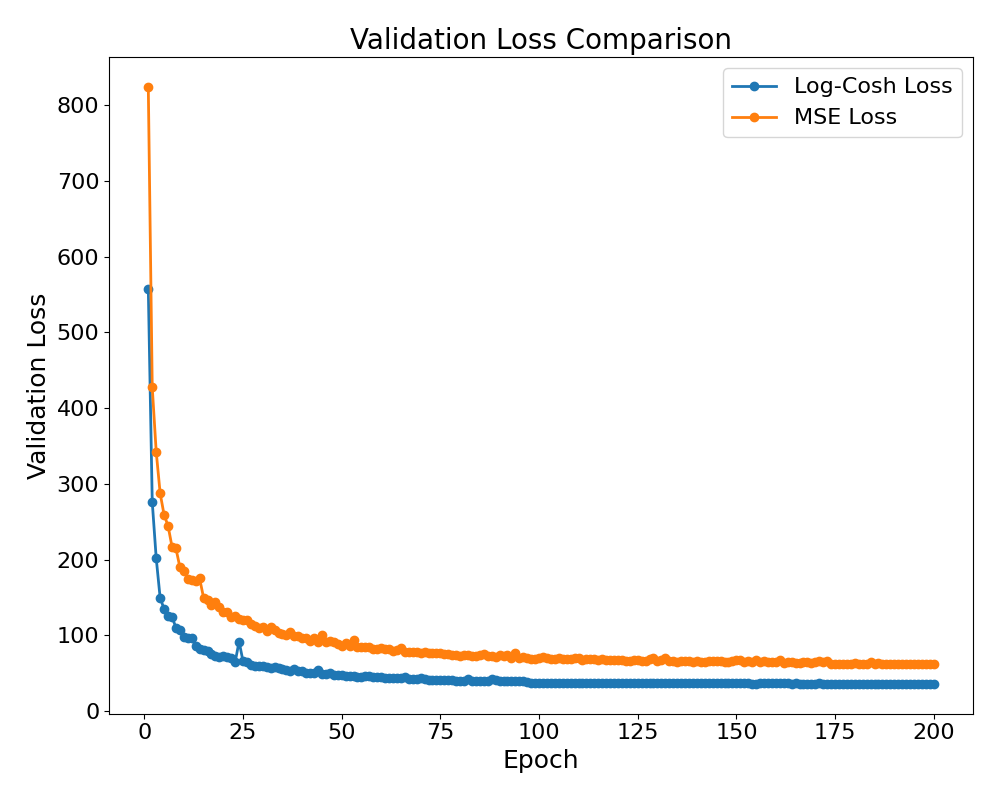
\includegraphics[width=\textwidth]{img/vae_results/val_loss_comparison.png}
        \caption{Validation Loss Comparison: Log-Cosh vs. MSE over all epochs.}
        \label{fig:val_loss_comparison}
    \end{subfigure}
    \hfill
    \begin{subfigure}[b]{0.49\textwidth}
        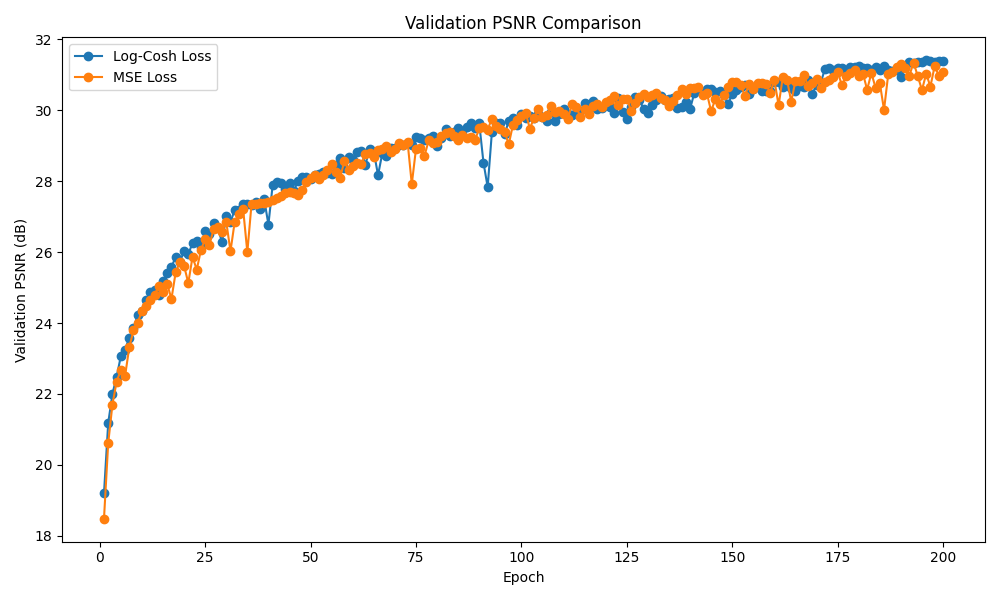
\includegraphics[width=\textwidth]{img/vae_results/val_psnr_comparison.png}
        \caption{Validation PSNR Comparison: Log-Cosh vs. MSE over all epochs.}
        \label{fig:val_psnr_comparison}
    \end{subfigure}
    
    \caption{Quantitative Comparison of Loss Functions: Validation Loss and PSNR for Log-Cosh and MSE variants.}
    \label{fig:quant_comparison}
\end{figure}


From these results:

\begin{itemize}
    \item The Log-Cosh loss outperformed MSE in terms of both total and reconstruction loss, indicating smoother training and better pixel-wise fidelity.
    \item A higher PSNR suggests improved perceptual quality in reconstructions when using Log-Cosh.
    \item KL Divergence was slightly lower for Log-Cosh, indicating a better balance between compression and regularization.
    \item These results affirm the hypothesis that the Log-Cosh loss leads to more visually realistic reconstructions, thus answering RQ2.
\end{itemize}



\subsection{Visual Comparison of Reconstructions} \label{subsubsec:vae_visual_recon}
Representative input images and corresponding reconstructions from both models at epoch 200 were visually compared.

Log-Cosh Reconstructions (Figure~\ref{fig:logcosh_epoch200}) retain road boundaries, tree textures, and lighting gradients with greater smoothness and fewer artifacts.

MSE Reconstructions (Figure~\ref{fig:mse_epoch200}) exhibit noise in edge regions and less coherent texture patterns and lost many important details like traffic light pole, road boundary and many more.

These qualitative results further confirms that adopting the Log-Cosh loss, as motivated by Chen et al.~\cite{chen2019log}, substantially improves VAE performance thereby answering RQ2 (How can loss function modifications in Variational Autoencoders (VAEs) optimize image reconstruction quality in autonomous driving tasks?).


%\vspace{1em}
\subsection{Latent Space Visualization and Separability} \label{subsubsec:vae_latent_space}

Beyond reconstruction fidelity, an essential aspect of the VAE's role in this thesis is to produce semantically rich and class-discriminative latent representations that can serve downstream classifiers and interpretability frameworks. To explore this, dimensionality reduction techniques were applied to the 128-dimensional latent vectors obtained from the test dataset using the final logcosh trained model.

Figures~\ref{fig:pca_true} and~\ref{fig:pca_pred} show the latent space compressed to two principal components using PCA, with each point color-coded by either the true class label or the classifier predicted label. The projections reveal clear and compact clusters for classes like \texttt{STOP} and \texttt{RIGHT}, while \texttt{GO} and \texttt{LEFT} appear more entangled suggesting potential ambiguities in those classes' feature space.

\begin{figure}[htbp]
    \centering
    \begin{subfigure}[b]{0.49\textwidth}
        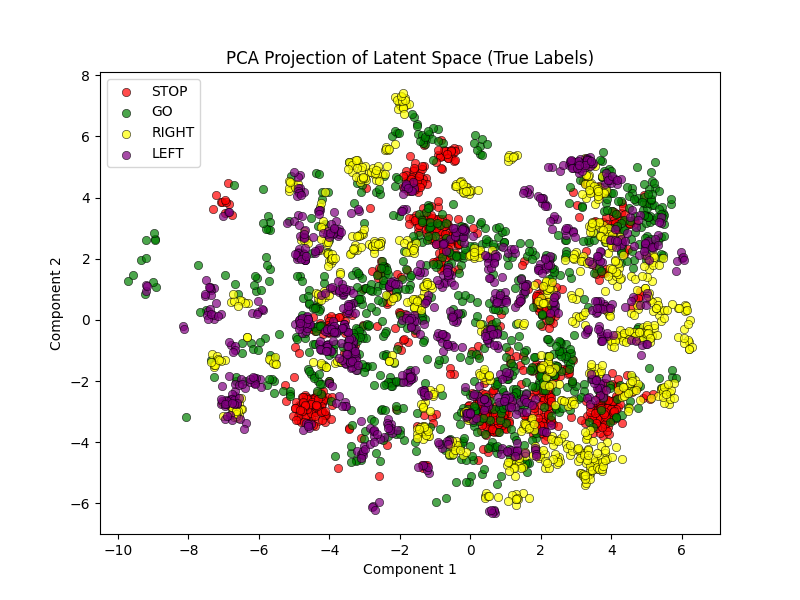
\includegraphics[width=\textwidth]{img/vae_results/pca_latent_space_true_labels.png}
        \caption{PCA projection of latent vectors from the test set, colored by true class labels.}
        \label{fig:pca_true}
    \end{subfigure}
    \hfill
    \begin{subfigure}[b]{0.49\textwidth}
        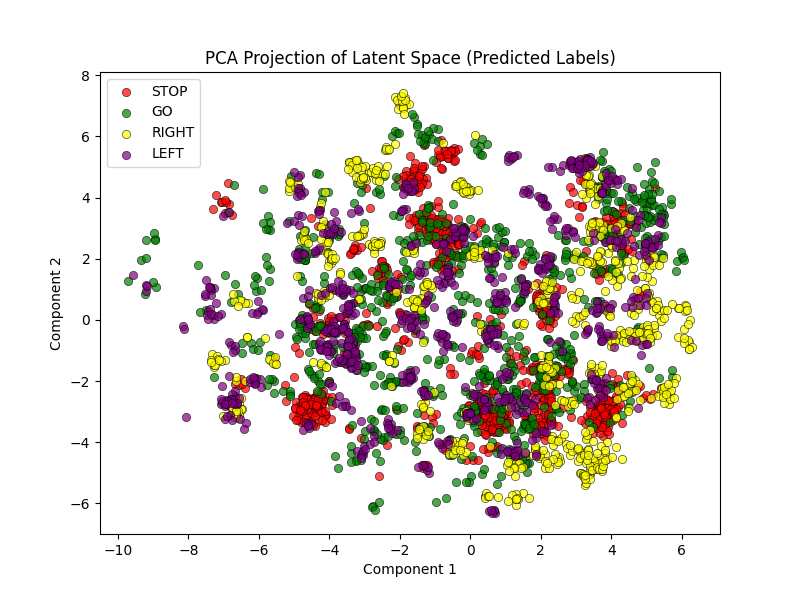
\includegraphics[width=\textwidth]{img/vae_results/pca_latent_space_predicted_labels.png}
        \caption{PCA projection of latent vectors, colored by classifier-predicted labels.}
        \label{fig:pca_pred}
    \end{subfigure}
\end{figure}

To uncover more nuanced non-linear relationships, t-SNE was applied. Figures~\ref{fig:tsne_true} and~\ref{fig:tsne_pred} visualize these embeddings, revealing denser local clusters and class-wise groupings that validate the VAE’s capacity to capture semantically meaningful structure—even without explicit supervision during training.

\begin{figure}[htbp]
    \centering
    \begin{subfigure}[b]{0.49\textwidth}
        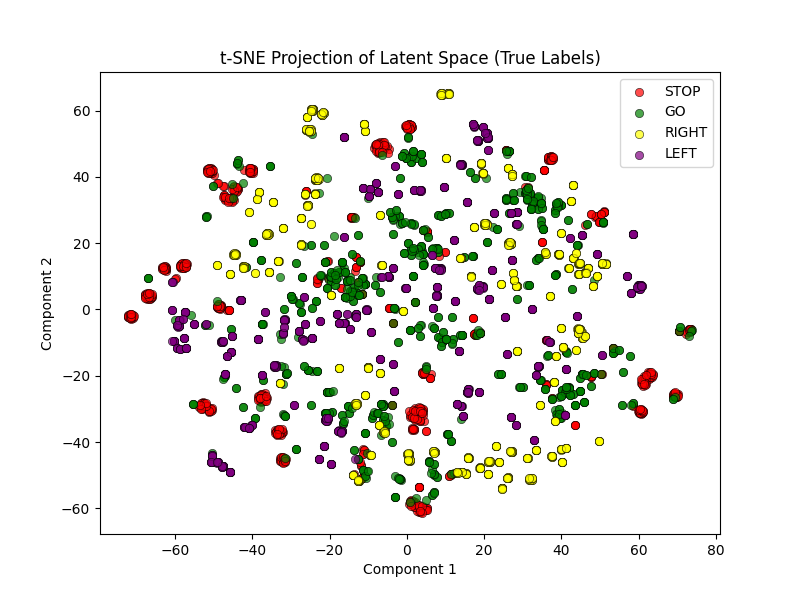
\includegraphics[width=\textwidth]{img/vae_results/tsne_latent_space_true_labels.png}
        \caption{t-SNE projection of latent space using true labels. Localized clustering is evident for most classes.}
        \label{fig:tsne_true}
    \end{subfigure}
    \hfill
    \begin{subfigure}[b]{0.49\textwidth}
        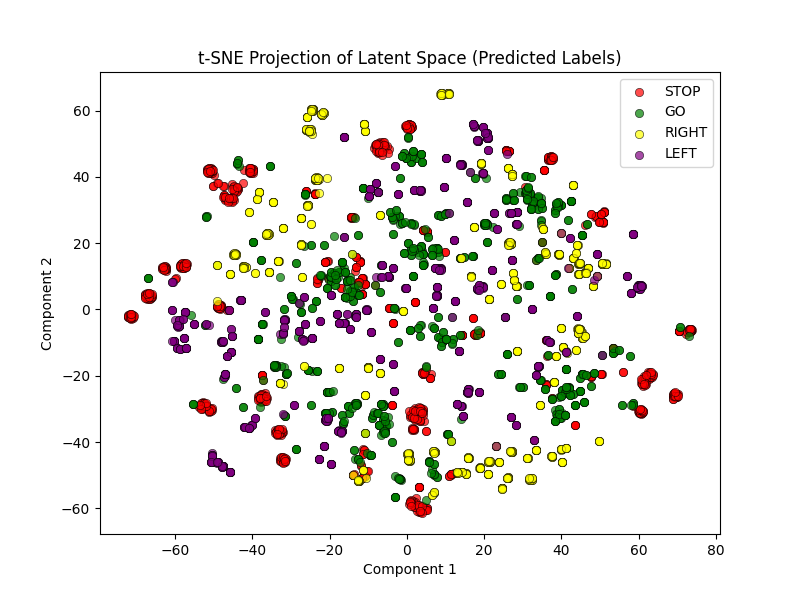
\includegraphics[width=\textwidth]{img/vae_results/tsne_latent_space_predicted_labels.png}
        \caption{t-SNE projection of latent space using predicted labels. Model-predicted clusters mirror semantic grouping.}
        \label{fig:tsne_pred}
    \end{subfigure}
\end{figure}

These visualizations Figures~\ref{fig:pca_true} and~\ref{fig:pca_pred}, and Figures~\ref{fig:tsne_true} and~\ref{fig:tsne_pred} indicate that the VAE latent space exhibits both global and local separability. While PCA suggests broad class groupings, t-SNE highlights fine-grained clusters. The relative alignment between true and predicted label distributions further confirms that the latent features are discriminative and conducive to effective classification.

This supports the hypothesis that the VAE encodes compact, informative, and semantically meaningful representations from high-dimensional input data, successfully addressing the goals of \textbf{RQ1}.










\section{Evaluation of Classifiers Trained on Latent Features} \label{sec:classifier_eval}

Following the successful design and training of the Variational Autoencoder (VAE), the next step in this thesis was to assess the effectiveness of its learned latent space in enabling downstream decision-making. Specifically, this section evaluates whether the encoded 128-dimensional latent representations can support accurate multi-class classification of driving actions. This directly addresses the core objective of \textbf{RQ1}, by investigating the semantic richness and discriminative power of the latent vectors produced by the VAE.

To this end, a set of traditional and neural classifiers were trained and evaluated on the same VAE-derived latent representations, using a balanced four-class dataset comprising \texttt{STOP}, \texttt{GO}, \texttt{LEFT}, and \texttt{RIGHT} labels. Five models were studied: Logistic Regression (baseline linear classifier), K-Nearest Neighbors (KNN), Random Forest (RF), Support Vector Machine (SVM), and Neural Network (NN).

Classifier training implementation details are described in \cref{sec:classifier_architectures}. Performance evaluation was carried out using a comprehensive set of metrics such as accuracy, per-class precision, recall, F1-score, macro and weighted averages, confusion matrices, and ROC-AUC curves for one-vs-rest classification~\cite{labelf2025metrics, roc_auc2024, svm_rf_knn2017}.



\subsection{Evaluations and Results of Traditional Classifiers} \label{subsec:comparision_with_traditional_classifiers}

To contextualize the performance of the neural model, four traditional classifiers were evaluated using the same latent vectors. Training and implementations of these classifiers are elaborated in \cref{sec:classifier_architectures}. Figure~\ref{fig:comparison_matrices} summarizes the confusion matrices for each model, and Figure~\ref{fig:comparison_rocs} provides the corresponding ROC curves.

\begin{figure}[h]
\centering
\begin{subfigure}{0.48\textwidth}
    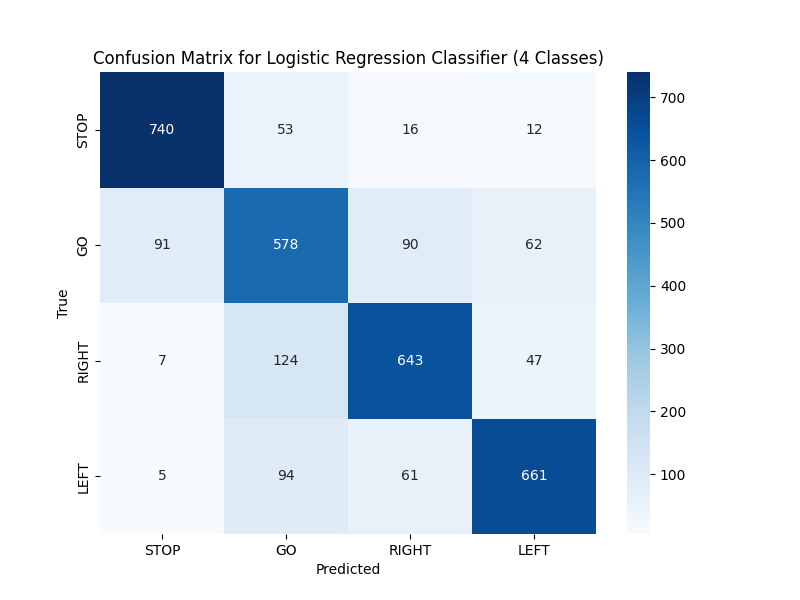
\includegraphics[width=\linewidth]{img/classifier/logistic_regression_confucion_matrix.png}
    \caption{Logistic Regression}
\end{subfigure}
\begin{subfigure}{0.48\textwidth}
    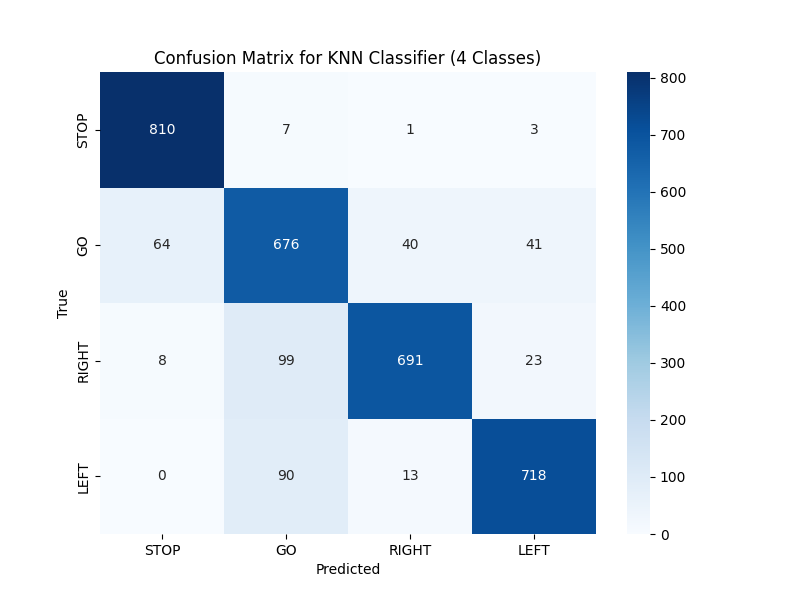
\includegraphics[width=\linewidth]{img/classifier/KNN_confucion_matrix.png}
    \caption{KNN}
\end{subfigure}

\vspace{0.5em}

\begin{subfigure}{0.48\textwidth}
    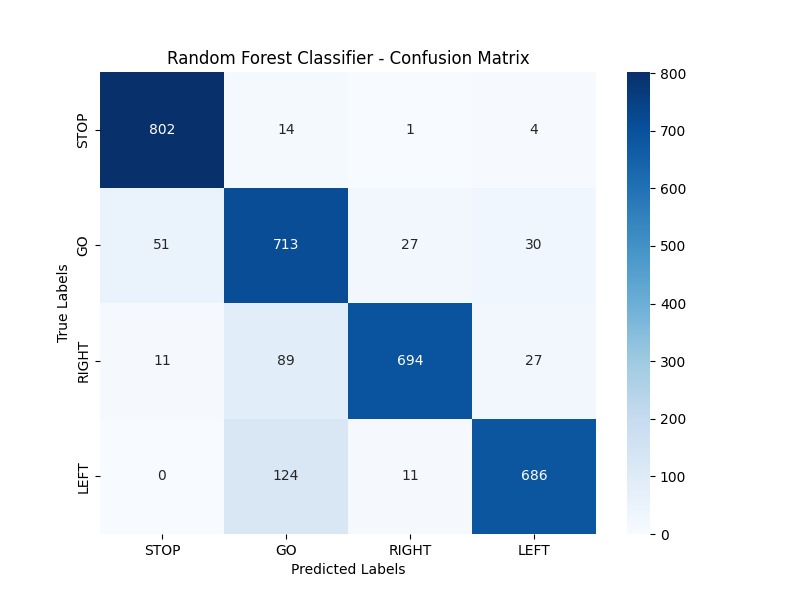
\includegraphics[width=\linewidth]{img/classifier/random_forest_confucion_matrix.png}
    \caption{Random Forest}
\end{subfigure}
\begin{subfigure}{0.48\textwidth}
    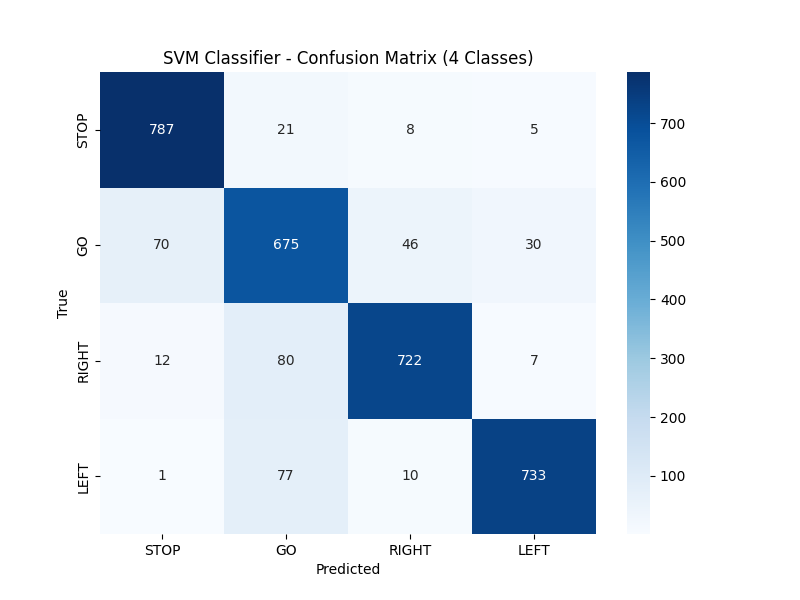
\includegraphics[width=\linewidth]{img/classifier/SVM_confucion_matrix.png}
    \caption{SVM}
\end{subfigure}

\caption{Confusion matrices for traditional classifiers.}
\label{fig:comparison_matrices}
\end{figure}


\begin{figure}[h]
\centering
\begin{subfigure}{0.48\textwidth}
    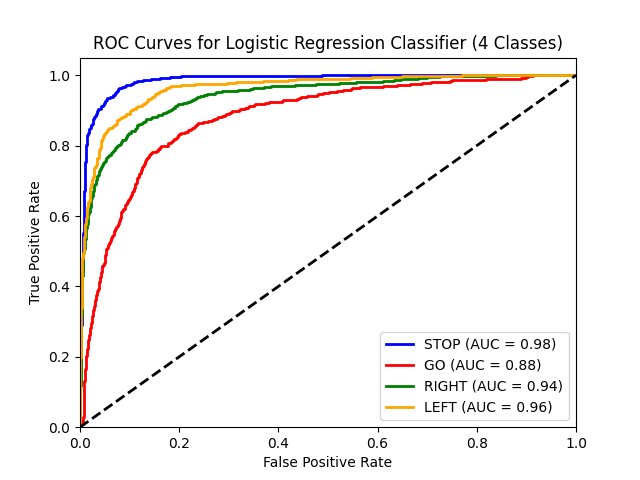
\includegraphics[width=\linewidth]{img/classifier/logistic_regression_AUC.png}
    \caption{Logistic Regression}
\end{subfigure}
\begin{subfigure}{0.48\textwidth}
    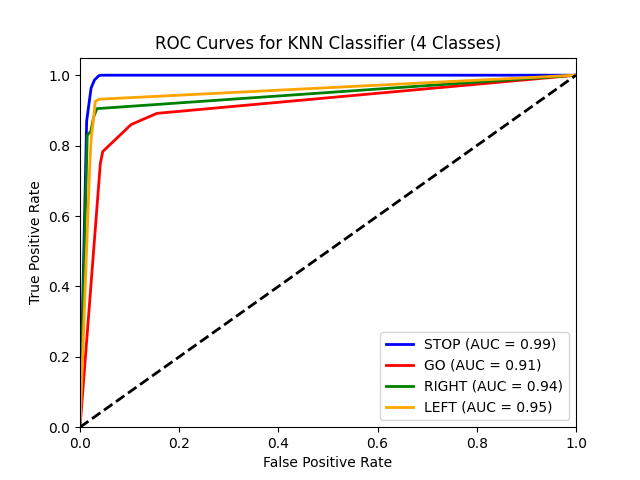
\includegraphics[width=\linewidth]{img/classifier/KNN_AUC.png}
    \caption{KNN}
\end{subfigure}

\vspace{0.5em}

\begin{subfigure}{0.48\textwidth}
    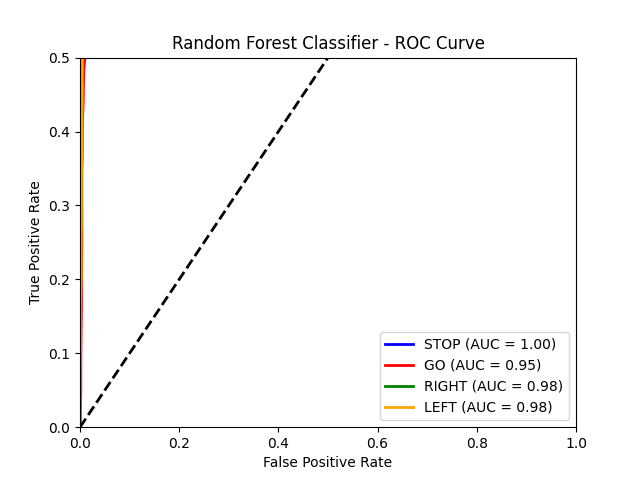
\includegraphics[width=\linewidth]{img/classifier/random_forest_AUC.png}
    \caption{Random Forest}
\end{subfigure}
\begin{subfigure}{0.48\textwidth}
    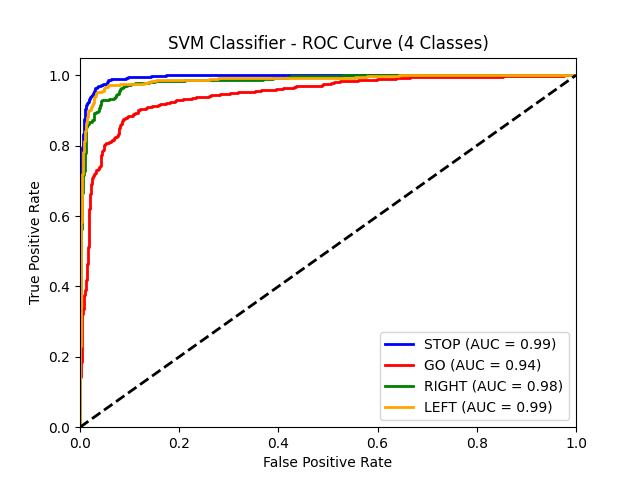
\includegraphics[width=\linewidth]{img/classifier/SVM_AUC.png}
    \caption{SVM}
\end{subfigure}

\caption{ROC curves and AUC values for traditional classifiers (1-vs-rest).}
\label{fig:comparison_rocs}
\end{figure}





\paragraph{Logistic Regression.}

The Logistic Regression classifier achieved an overall accuracy of 80\% and a macro F1-score of 0.80. As seen in Figure~\ref{fig:comparison_matrices}(a), the confusion matrix reveals that the model performs well for the \texttt{STOP} and \texttt{LEFT} classes, while showing significant misclassification for the \texttt{GO} and \texttt{RIGHT} classes. Notably, many \texttt{GO} instances were misclassified as \texttt{RIGHT} or \texttt{LEFT}, highlighting the difficulty in linearly separating these features in the latent space.

The ROC curves in Figure~\ref{fig:comparison_rocs}(a) further support this observation. While the \texttt{STOP} and \texttt{LEFT} classes achieved high AUC scores (0.98 and 0.96 respectively), the \texttt{GO} class recorded the lowest AUC at 0.88, indicating a higher overlap with other classes in the latent space.

Overall, Logistic Regression acts as a valuable baseline. Its performance confirms the need for non-linear classifiers to fully leverage the representational power of the VAE's latent space.

\paragraph{K-Nearest Neighbors (KNN).}

The K-Nearest Neighbors classifier achieved an overall accuracy of 88\% and a macro F1-score of 0.88, demonstrating competitive performance on the latent feature space extracted by the VAE. As shown in Figure~\ref{fig:comparison_matrices}(b), the model achieved near-perfect recall for the \texttt{STOP} class (99\%) and high precision for both \texttt{STOP} and \texttt{RIGHT}.

The most significant confusion occurred between the \texttt{LEFT} and \texttt{GO} classes, where 92 instances of \texttt{LEFT} were incorrectly predicted as \texttt{GO}, likely due to local similarity in features. This aligns with the proximity-based nature of KNN, which is sensitive to cluster overlap in high-dimensional spaces.

Figure~\ref{fig:comparison_rocs}(b) shows the ROC curves, where all classes achieve AUC values above 0.90. \texttt{STOP} reached the highest AUC of 0.99, followed by \texttt{LEFT} (0.95), \texttt{RIGHT} (0.94), and \texttt{GO} (0.91).

In summary, KNN offers a strong non-parametric baseline that effectively captures local structure in the VAE's latent space, though it may require further tuning or metric learning to fully disambiguate overlapping action classes.


\paragraph{Random Forest.}
The Random Forest classifier achieved an accuracy of 88\% and a macro F1-score of 0.88. As shown in Figure~\ref{fig:comparison_matrices}(c), the confusion matrix indicates strong performance across most classes, particularly for \texttt{STOP} (F1 = 0.95) and \texttt{RIGHT} (F1 = 0.89). The model also demonstrated competitive recall for the \texttt{GO} class (0.87), which often presents the most overlap with other categories.

ROC analysis (Figure~\ref{fig:comparison_rocs}(c)) revealed high AUC scores across the board, with \texttt{STOP} achieving a perfect AUC of 1.00, and the other classes maintaining AUCs above 0.95. These findings affirm the Random Forest’s ability to exploit the structure of the latent space effectively.

Complete classification metrics for all four classes are provided in Appendix~\ref{tab:random_forest_classification_report}, which reinforce the model’s balanced precision and recall across classes.

\paragraph{Support Vector Machine (SVM).}
The SVM classifier achieved an overall accuracy of 89\% and a macro F1-score of 0.89, outperforming several traditional models. As seen in Figure~\ref{fig:comparison_matrices}(d), the confusion matrix reveals strong and consistent performance across all classes. The model performed especially well for \texttt{STOP} and \texttt{LEFT} classes with F1-scores of 0.93 and 0.92 respectively, and demonstrated solid performance for \texttt{RIGHT} (F1 = 0.90). While the \texttt{GO} class had slightly lower scores (F1 = 0.81), it still surpassed performance seen in Logistic Regression and KNN.

The ROC curves in Figure~\ref{fig:comparison_rocs}(d) further support this, showing high AUC values across all classes, each reaching or exceeding 0.94. This indicates excellent class separability in the latent space when using a margin-based classifier with non-linear kernels.

A detailed breakdown of the classification metrics is available in Appendix~\ref{tab:svm_classification_report}, demonstrating that SVMs can leverage the non-linear separability embedded in the latent representations learned by the VAE.




Table~\ref{tab:classifier_comparison} presents a side-by-side comparison of accuracy and F1-scores across all classifiers:

\begin{table}[htbp]
\centering
\small
\begin{tabular}{p{3cm}ccp{5.5cm}}
\toprule
\textbf{Classifier} & \textbf{Accuracy} & \textbf{Macro F1} & \textbf{Notes} \\
\midrule
Logistic Regression & 80\% & 0.80 & Baseline linear classifier; struggled with \texttt{GO} \\
KNN & 88\% & 0.88 & High recall for \texttt{STOP}; sensitive to latent proximity \\
SVM & 89\% & 0.89 & Excellent class separability; strong on \texttt{LEFT} and \texttt{STOP} \\
Random Forest & 88\% & 0.88 & Robust performance; most errors in \texttt{GO} class \\
Neural Network & \textbf{89\%} & \textbf{0.89} & Best overall F1 balance; handles non-linear separations \\
\bottomrule
\end{tabular}
\caption{Performance comparison of classifiers trained on VAE latent features (4-class).}
\label{tab:classifier_comparison}
\end{table}


Across all classifiers, the \texttt{GO} class consistently had the lowest precision and recall. This suggests latent encodings for \texttt{GO} overlap more with other classes, possibly due to its transitional visual nature. Addressing this may require additional context, or spatial features.


\subsection{Evaluation of Neural Network Classifier (MLP)}
\label{subsec:classifier_trained_on_latentfeatures}

The neural network classifier, implemented as a Multi-Layer Perceptron (MLP), was trained for 20 epochs on the 128-dimensional latent features extracted from the VAE encoder. This model aimed to capture the non-linear relationships within the latent space and serve as a powerful baseline for downstream classification tasks.

Training progression is visualized in Figure~\ref{fig:loss_accuracy_plot}, which shows the learning dynamics over the course of training. The left plot demonstrates a consistent reduction in loss, while the right plot shows a steady increase in training accuracy, reaching a final value of approximately 93\%. These curves indicate effective convergence without overfitting, affirming the model's ability to generalize well on latent representations.

\begin{figure}[h]
    \centering
    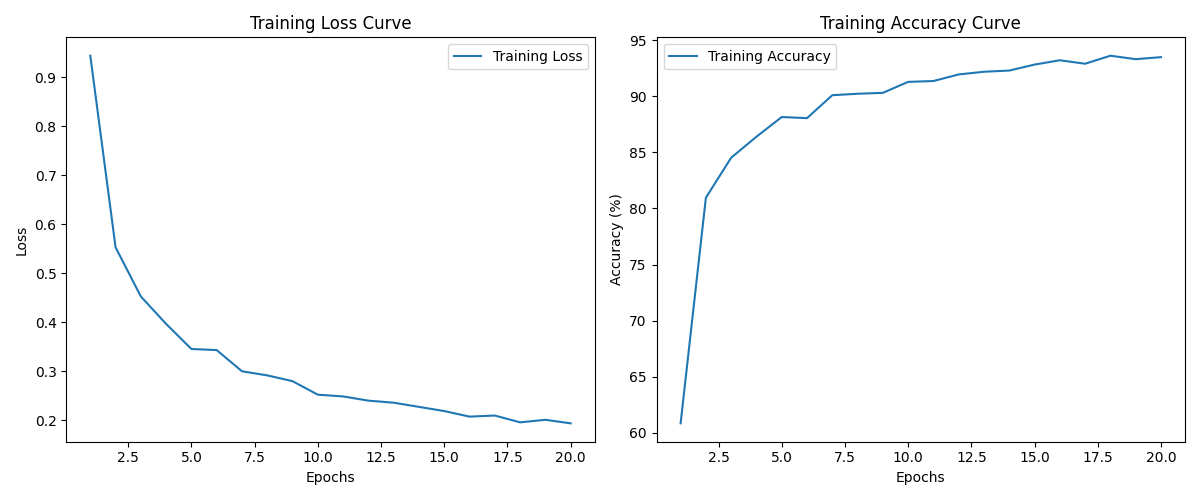
\includegraphics[width=\textwidth]{img/classifier/training_loss_accuracy_4_classes.png}
    \caption{Training loss and accuracy curves for the neural classifier over 20 epochs.}
    \label{fig:loss_accuracy_plot}
\end{figure}

Quantitative evaluation results on the test set are presented in Table~\ref{tab:classification_report}. The MLP achieved an overall accuracy of 89\% and a macro-averaged F1-score of 0.89, demonstrating robust performance across all four driving behavior classes.

\begin{table}[h]
    \centering
    \begin{tabular}{lcccc}
        \toprule
        \textbf{Class} & \textbf{Precision} & \textbf{Recall} & \textbf{F1-score} & \textbf{Support} \\
        \midrule
        STOP & 0.91 & 0.99 & 0.95 & 821 \\
        GO & 0.81 & 0.84 & 0.83 & 821 \\
        RIGHT & 0.93 & 0.86 & 0.89 & 821 \\
        LEFT & 0.93 & 0.89 & 0.91 & 821 \\
        \midrule
        \textbf{Accuracy} & \multicolumn{4}{c}{0.89 (3284 samples)} \\
        \textbf{Macro avg} & 0.90 & 0.89 & 0.89 & -- \\
        \textbf{Weighted avg} & 0.90 & 0.89 & 0.89 & -- \\
        \bottomrule
    \end{tabular}
    \caption{Classification report for the neural network trained on latent features (4-class).}
    \label{tab:classification_report}
\end{table}

The confusion matrix in Figure~\ref{fig:conf_matrix} provides additional insights into the model's performance by revealing class-specific error patterns. The \texttt{STOP} class is classified with the highest precision and recall, while the \texttt{GO} class remains the most challenging due to its visual and contextual overlap with other classes.

\begin{figure}[h]
    \centering
    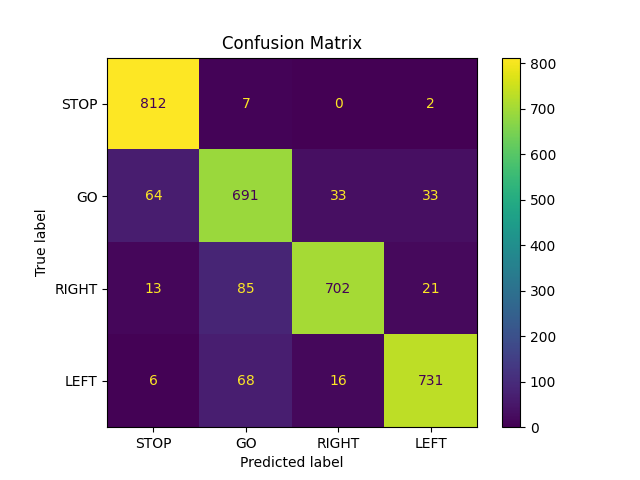
\includegraphics[width=0.6\textwidth]{img/classifier/confusion_matrix_4_classes.png}
    \caption{Confusion matrix for the neural classifier on the 4-class test set.}
    \label{fig:conf_matrix}
\end{figure}

\begin{itemize}
    \item \textbf{STOP:} Most accurately classified class (Recall = 0.99), confirming its strong separability in the latent space.
    \item \textbf{GO:} Lowest-performing class with Precision = 0.81 and Recall = 0.84. Common misclassifications include confusion with \texttt{RIGHT} and \texttt{LEFT}.
    \item \textbf{RIGHT:} High precision (0.93) and moderate recall (0.86). Some misclassification occurs with the \texttt{GO} class.
    \item \textbf{LEFT:} Balanced performance with strong metrics across all dimensions, but minor confusion with \texttt{GO} was observed.
\end{itemize}

These results suggest that the learned latent space is semantically meaningful and well-structured, enabling accurate and efficient multi-class classification. The MLP outperformed all traditional classifiers, confirming the hypothesis that non-linear models are better suited for leveraging the representational richness of the VAE-derived latent features. This conclusion directly supports the research question RQ1 regarding the effectiveness of latent representations for downstream prediction.

\begin{itemize}
    \item \textbf{Neural Classifier and SVM} emerged as top performers, both achieving an F1-score of 0.89 and high recall for critical classes such as \texttt{STOP} and \texttt{LEFT}.
    \item \textbf{Random Forest} performed competitively, with strong recall on \texttt{STOP} (0.98), but showed minor confusion on \texttt{GO} and \texttt{LEFT}.
    \item \textbf{KNN} offered fast implementation with solid results, but is sensitive to feature scaling and suffered from overlap in ambiguous classes like \texttt{GO}.
    \item \textbf{Logistic Regression} showed the weakest performance (Accuracy = 80\%), revealing the limitations of linear separability in the VAE's latent space.
\end{itemize}

\subsection{Discussion of Classifier Results}

This comprehensive evaluation confirms that the latent space learned by the VAE is highly effective for downstream classification tasks. All classifiers achieved reasonable performance with macro F1-scores above 0.80. However, the Neural Network (MLP) classifier consistently outperformed other models in terms of both accuracy and generalization across all four driving classes. With an F1-score of 0.89 and robust recall on all classes—including the more ambiguous ones like GO and LEFT the MLP demonstrated superior capability in modeling the non-linear structure of the VAE's latent space.

While SVM and Random Forest showed competitive performance, their training flexibility and scalability were limited compared to the MLP, especially when extended to gradient-based counterfactual explanation methods. KNN and Logistic Regression served as valuable baselines but lacked the expressive power required for capturing complex class boundaries in the latent space.

Therefore, the MLP classifier was selected for all downstream experiments and counterfactual explanation tasks throughout this thesis. Its deep architecture, non-linear activation functions, and regularization mechanisms make it particularly well-suited for high-dimensional, semantically rich latent features generated by the VAE. This choice ensures consistency, interpretability, and compatibility with the explanation frameworks introduced in later chapters.

These findings empirically support the hypothesis posed in RQ1 that deep generative models like VAEs can produce compact yet semantically meaningful representations of high-dimensional driving scenes representations that can be effectively leveraged for interpretable and reliable decision-making pipelines.









\section{Evaluation of Counterfactual Explanation Generation via Masking Techniques (RQ3)} \label{sec:masking_eval}
To address \textbf{RQ3}, we performed a comprehensive evaluation of all implemented masking techniques across multiple dimensions counterfactual coverage, computational efficiency, method overlap, and robustness. While object detection masking was initially considered, it was excluded from overlap analysis due to low detection rates and missed regions in the current dataset, resulting in poor counterfactual explanation coverage.

\subsection{Counterfactual Generation Coverage}
We first measured the number of successful counterfactuals generated by each masking method across the binary and multi-class datasets. Figures~\ref{fig:ce_count_binary} and \ref{fig:bar_chart_ce_count_multi} illustrate the total number of counterfactual explanations generated by each method, respectively.

\begin{figure}[htbp]
    \centering
    \begin{subfigure}{0.45\textwidth}
        \centering
        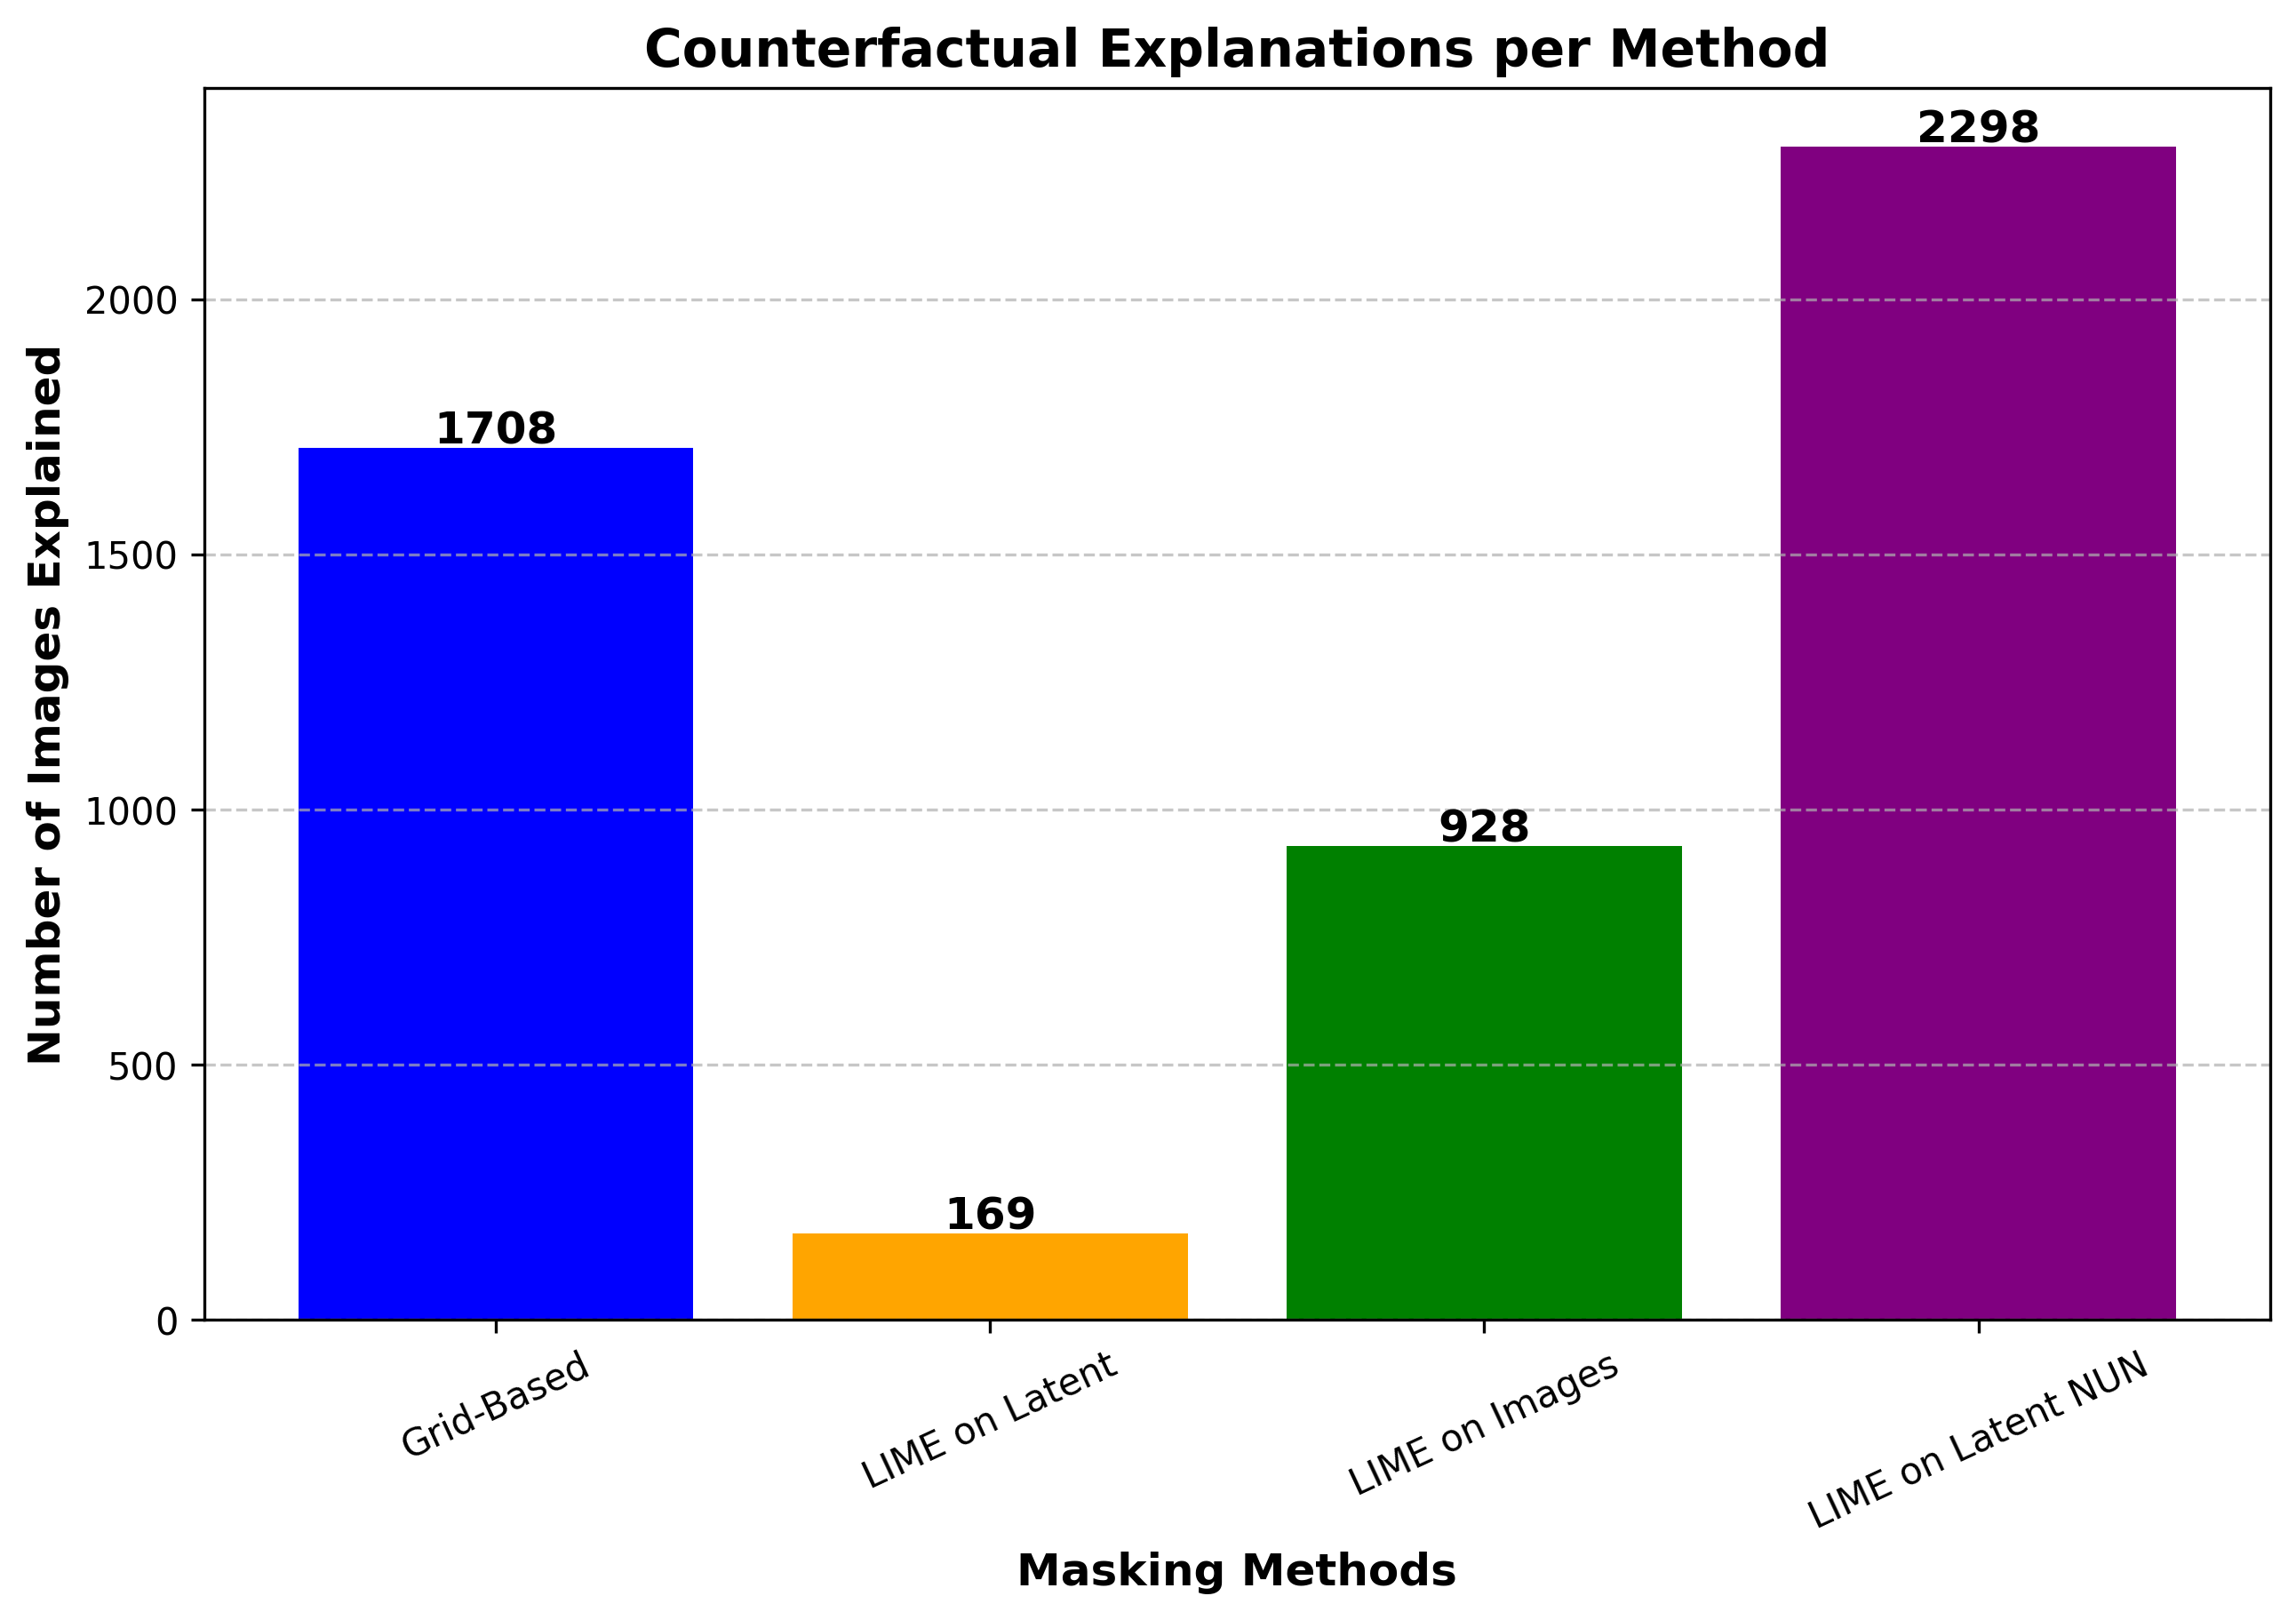
\includegraphics[width=\textwidth]{img/masking_results/bar_chart_explanations_2_class.png}
        \caption{Total number of counterfactual explanations generated by each method (2-class setup).}
        \label{fig:ce_count_binary}
    \end{subfigure}
    \hfill
    \begin{subfigure}{0.45\textwidth}
        \centering
        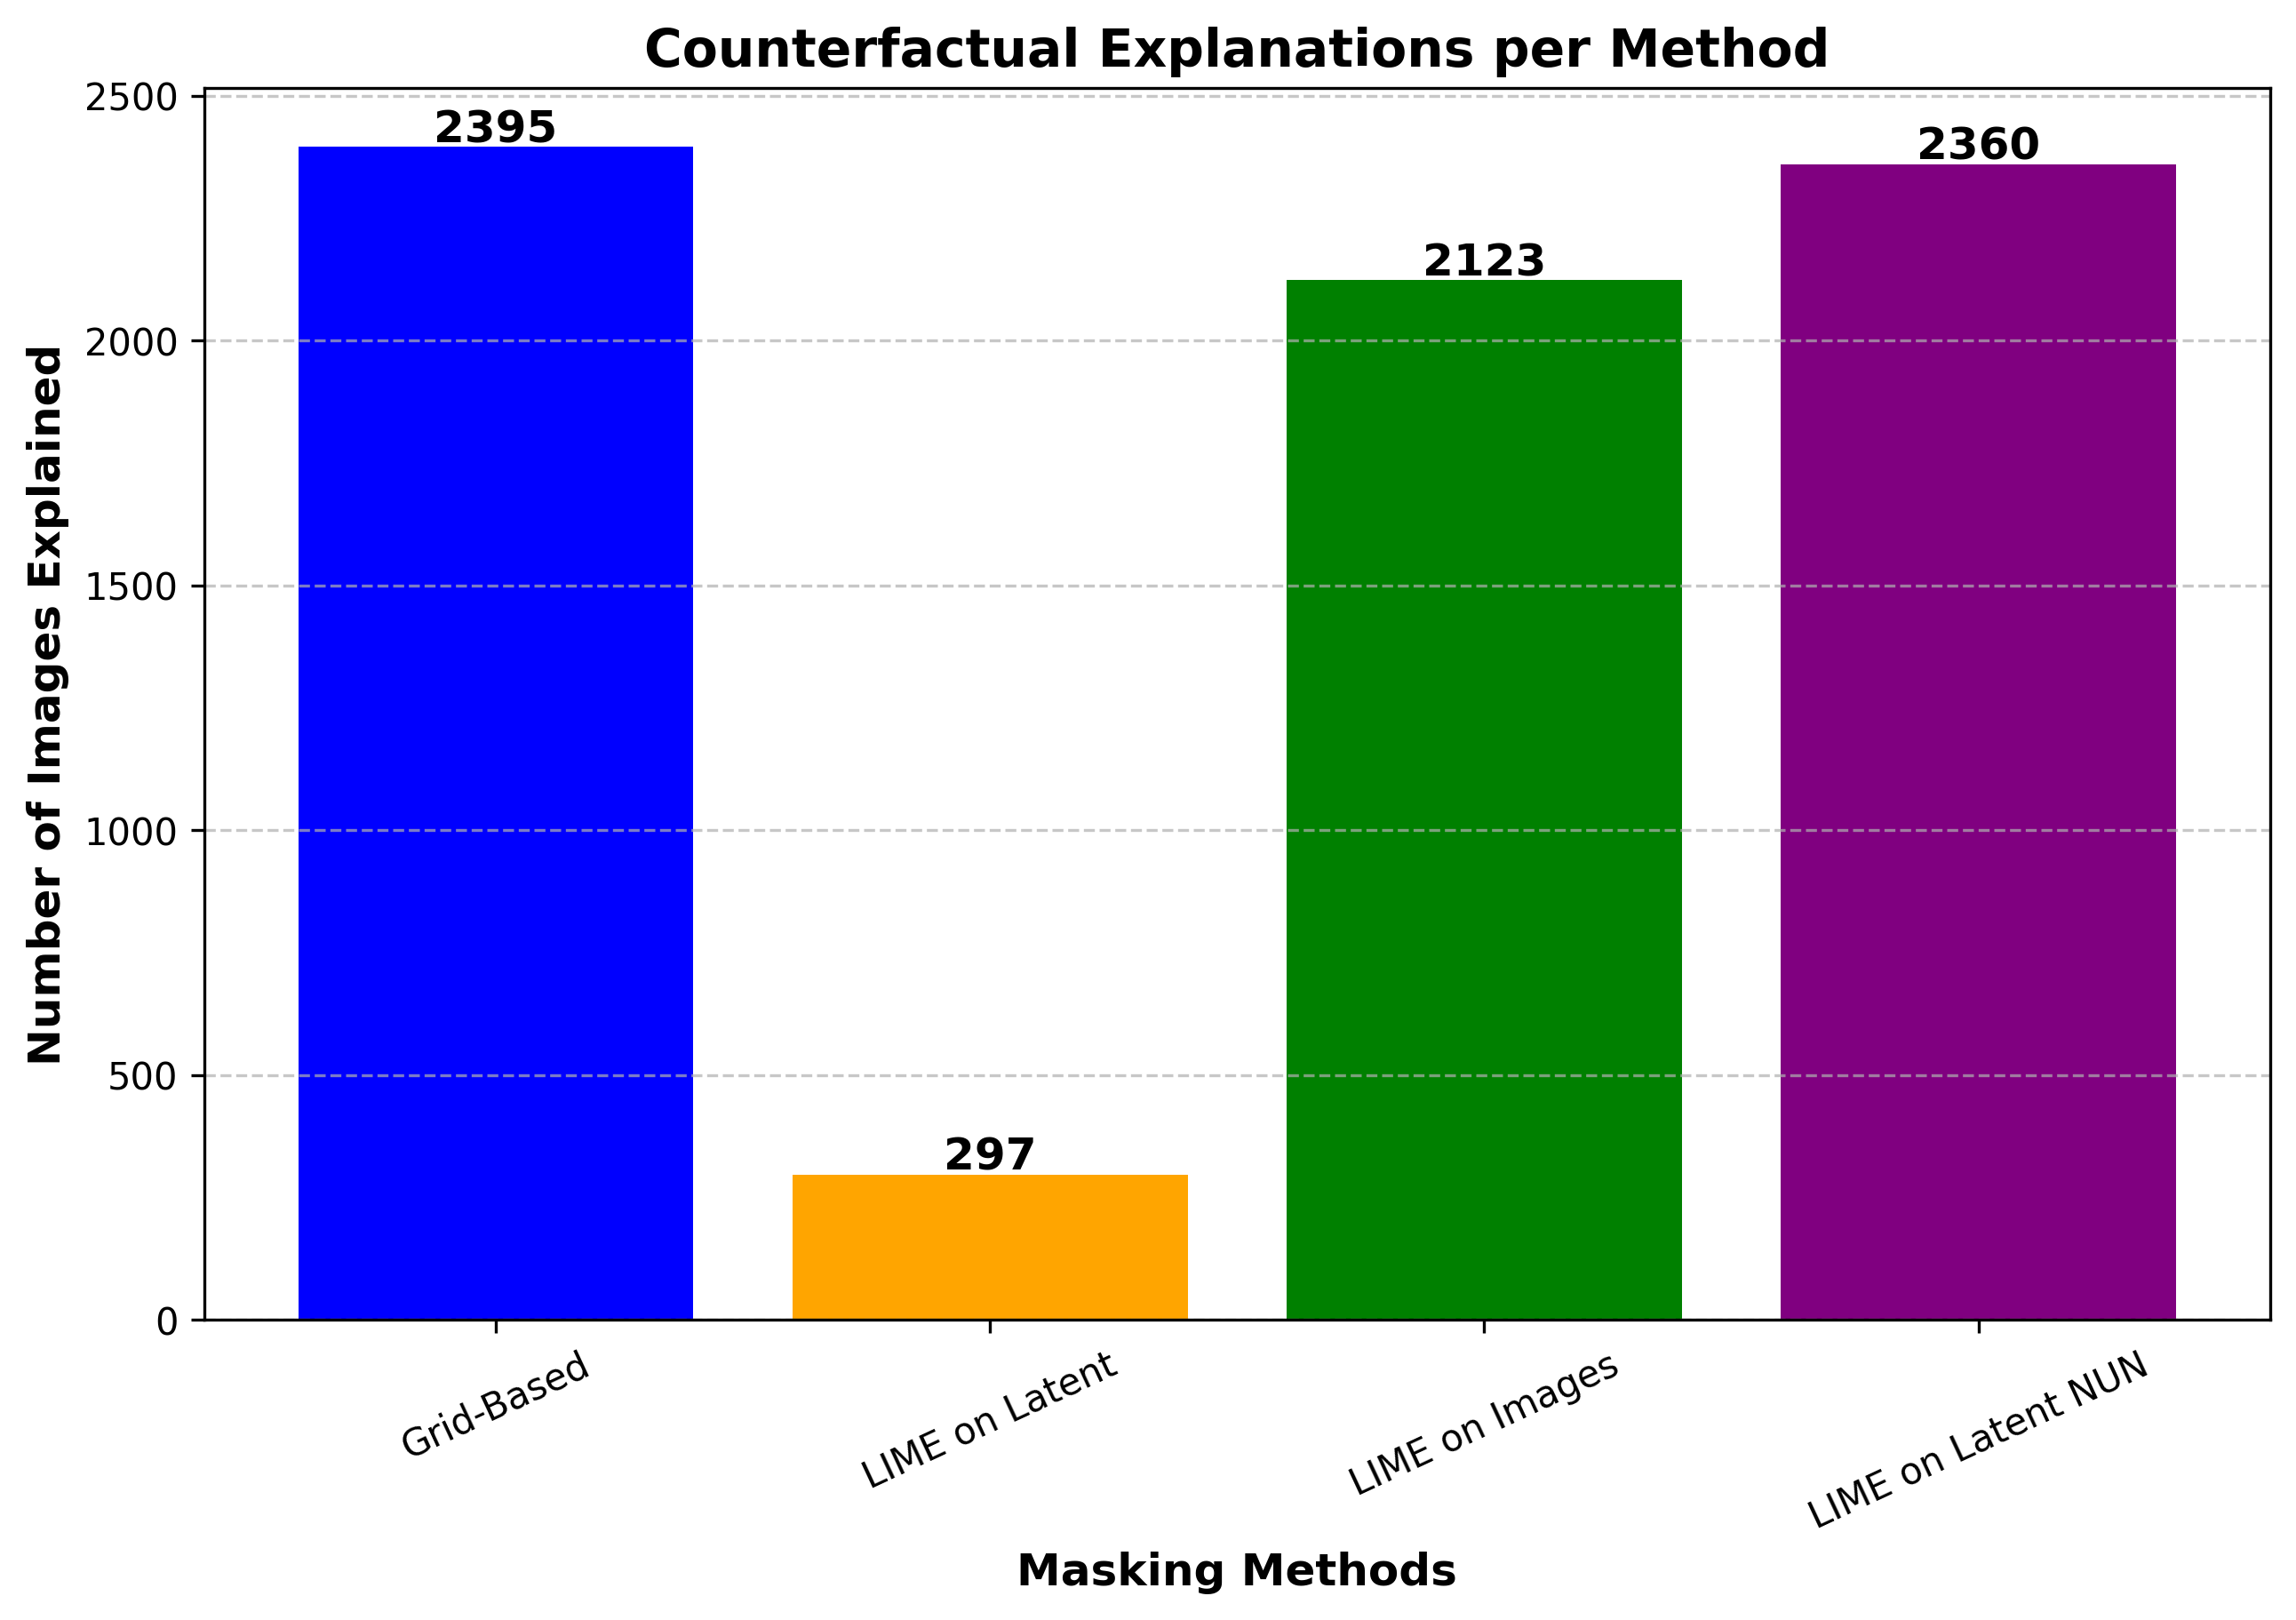
\includegraphics[width=\textwidth]{img/masking_results/bar_chart_explanations_4_class.png}
        \caption{Total number of counterfactual explanations generated by each method (4-class setup).}
        \label{fig:bar_chart_ce_count_multi}
    \end{subfigure}
    \caption{Comparison of counterfactual explanations generated by different masking methods.}
    \label{fig:ce_count_comparison}
\end{figure}

As shown in these figures, LIME on Latent NUN outperforms other methods in binary class and grid based maskning in multi-class settings. It successfully explained 2,298 out of 2,422 images (94.88\%) in the binary setup. While 2,395 images out of 2422 images (98.88\%) in the 4-class case. In contrast, LIME on Latent feature masking using median values shows the lowest performance, with only 6.98\% and 12.26\% success in the binary and multi-class settings, respectively.

\subsection{Masking Method Overlap} \label{subsubsec:masking_method_overlap}
To understand how these methods complement one another, we analyzed the overlaps in counterfactual explanations using Venn diagrams.

\begin{figure}[htbp]
    \centering
    \begin{subfigure}{0.45\textwidth}
        \centering
        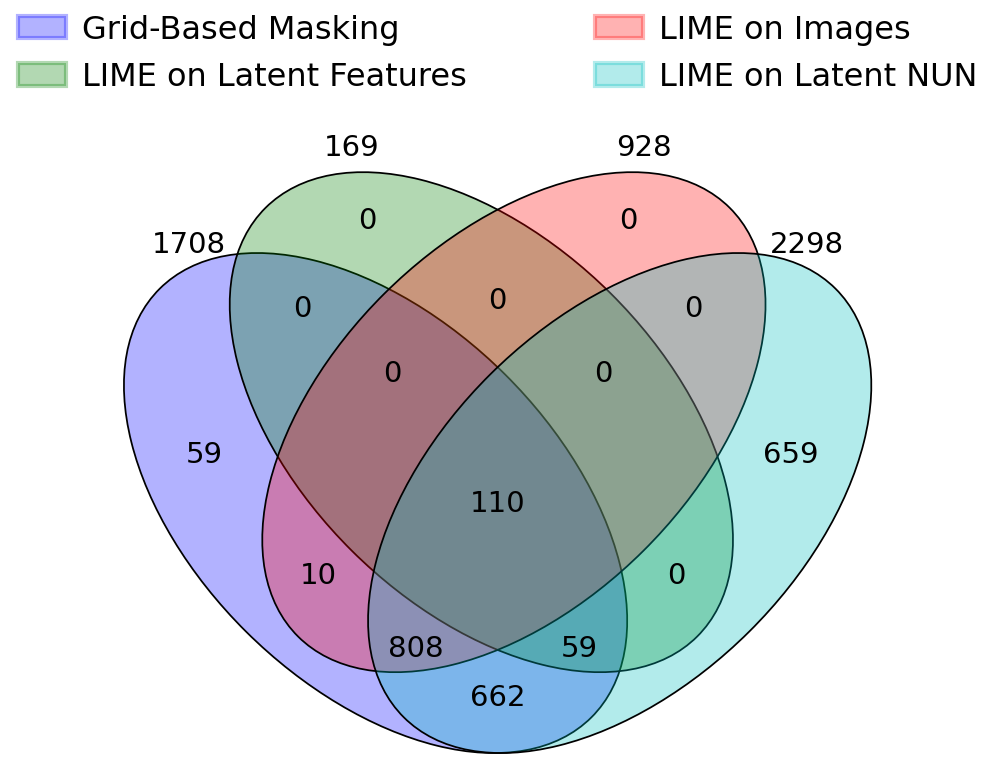
\includegraphics[width=\textwidth]{img/masking_results/venn_2_class.png}
        \caption{Venn diagram of counterfactual explanations by method (2-class setup).}
        \label{fig:venn_binary}
    \end{subfigure}
    \hfill
    \begin{subfigure}{0.45\textwidth}
        \centering
        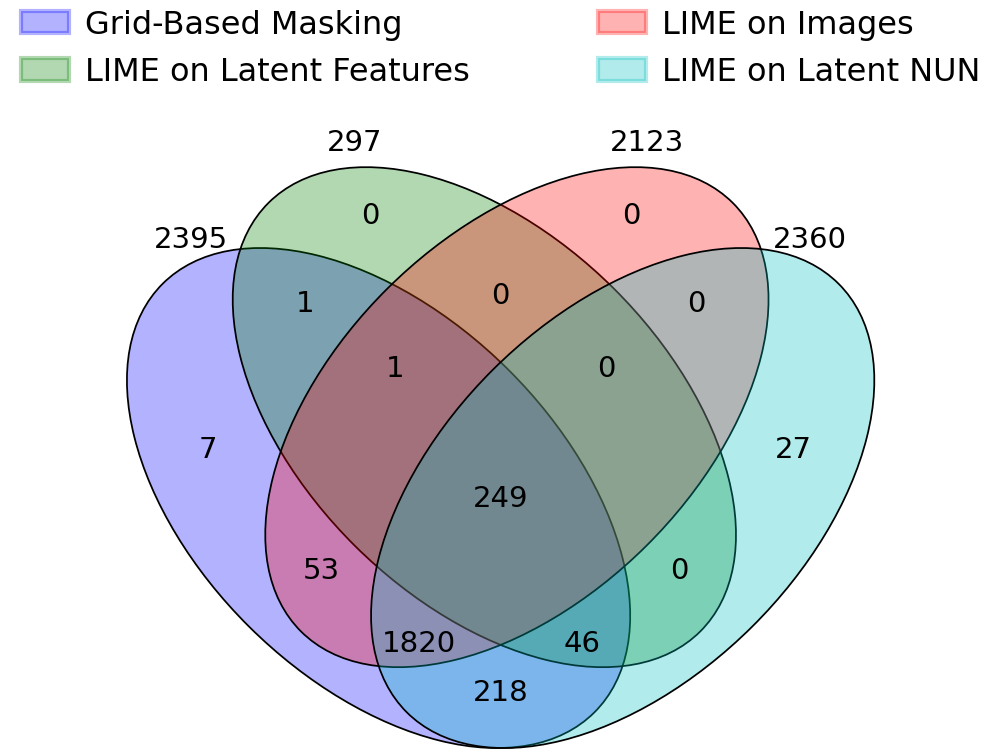
\includegraphics[width=\textwidth]{img/masking_results/venn_4_class.png}
        \caption{Venn diagram of counterfactual explanations by method (4-class setup).}
        \label{fig:venn_multi}
    \end{subfigure}
    \caption{Comparison of counterfactual explanations by method using Venn diagrams.}
    \label{fig:venn_comparison}
\end{figure}

From Figure~\ref{fig:venn_binary}, we observe:
\begin{itemize}
    \item 808 images (33.36\%) are explained by Grid-Based, LIME on Images, and LIME on Latent NUN masking methods together.
    \item 110 images (4.54\%) are explained by all four methods.
    \item 659 images (27.21\%) are exclusively explained by LIME on Latent NUN masking method.
\end{itemize}

Similarly, Figure~\ref{fig:venn_multi} reveals:
\begin{itemize}
    \item 1,820 images (75.14\%) are explained by Grid-Based, LIME on Images, and LIME on Latent NUN together.
    \item Only 249 images (10.28\%) are consistently explained by all four techniques.
\end{itemize}

These results indicate that while LIME on Latent feature masking contributes marginally when used alone, the LIME on Latent features masking using NUN method technique not only achieves broad coverage but also offers unique explanations not captured by other methods.


\subsection{Validity of Counterfactual Explanations}
Table~\ref{tab:ce_validity} presents the percentage of valid counterfactuals per masking method---i.e., cases where the predicted class changed post-masking while maintaining high-quality reconstruction. In this work, a counterfactual is considered valid if it alters the model’s output to the desired target class (e.g., from \texttt{STOP} to \texttt{GO}, or from \texttt{RIGHT} to \texttt{LEFT}).

The validity percentage is computed using the following formula:

\[
\text{Validity (\%)} = \left( \frac{\text{Successful Counterfactuals}}{\text{Total Counterfactuals}} \right) \times 100.
\]

\begin{table}[htbp]
\centering
\resizebox{\textwidth}{!}{%
\begin{tabular}{lccc}
\toprule
\textbf{Method} & \textbf{Binary CE Validity (\%)} & \textbf{Multi-Class CE Validity (\%)} & \textbf{Interpretation} \\
\midrule
Grid-Based Masking & 70.52 & 98.89 & Robust and fast; excellent for multi-class \\
LIME on Latent Maksing   & 6.98  & 12.26 & Limited effect, likely due to poor latent locality \\
LIME on Image Maksing    & 38.32 & 87.65 & Effective but slower due to pixel masking \\
LIME on Latent NUN& \textbf{94.88} & \textbf{97.44} & Highest performance and generalizability \\
\bottomrule
\end{tabular}%
}
\caption{Comparison of counterfactual explanation validity across masking methods.}
\label{tab:ce_validity}
\end{table}

These findings indicate that LIME on Latent NUN based masking is consistently effective across both binary and multi-class settings. The Grid-Based method performs well in multi-class but is less effective in binary scenarios when finer granularity is required.


\subsection{Per-Class Counterfactual Explanantions Success}
Table~\ref{tab:classwise_ce_multi} reports the number of valid counterfactuals generated per class.

\begin{table}[htbp]
\centering
\scriptsize
\begin{tabular}{lcccccccc}
\toprule
\textbf{Method} & \textbf{STOP (\%)} & \textbf{GO (\%)} & \textbf{LEFT (\%)} & \textbf{RIGHT (\%)} & \textbf{Total CE Found} & \textbf{Total CE (\%)} & \textbf{Total Time (min)} \\
\midrule
Grid-Based        & 100.0 & 100.0 & 89.0  & 100.0 & 2395 & 98.89 & 12.98 \\
LIME on Latent    & 10.3  & 9.4   & 18.4  & 26.1  & 297  & 12.26 & 92.63 \\
LIME on Image     & 100.0 & 100.0 & 1.6   & 74.5  & 2123 & 87.65 & 78.65 \\
LIME on Latent NUN & 98.6  & 96.0  & 97.2  & 99.6  & \textbf{2360} & \textbf{97.44} & 263.79 \\
\bottomrule
\end{tabular}
\caption{Per-class counterfactual explanation success (multi-class setup).}
\label{tab:classwise_ce_multi}
\end{table}

The table shows that while most methods effectively capture STOP and GO transitions, LIME on Latent NUN exhibits the most balanced performance across all classes, closely followed by the Grid-Based method.

\subsection{Visual Quality of Counterfactual Explanations} \label{subsec:visual_quality}
In addition to quantitative metrics such as coverage and class validity, we evaluated the perceptual quality of generated counterfactuals using Structural Similarity Index (SSIM) and Peak Signal-to-Noise Ratio (PSNR). These metrics measure how visually and structurally close the reconstructed image is to the original, thus reflecting the semantic plausibility of the explanation.

Figures~\ref{fig:ssim_boxplot} and \ref{fig:psnr_boxplot} present the box plots for SSIM and PSNR across the different masking techniques.

LIME on Latent feature masking using NUN method, LIME on Latent feature masking, and Grid-Based masking methods show high SSIM values (above 0.7) and PSNR in the 25--30 dB range, indicating sharp, semantically meaningful reconstructions. In contrast, LIME on Images results in low SSIM and PSNR due to zero-masking of important regions, which severely disrupts VAE reconstruction quality. These reconstructions often appear blurry or distorted. Object Detection-based masking shows moderate SSIM and PSNR, with high variance attributed to unreliable object detection results.


Overall, LIME on Latent NUN not only achieves high counterfactual success but also preserves image quality, making it suitable for interpretable and user-trustworthy explanations in real-world scenarios.


\begin{figure}[htbp]
    \centering
    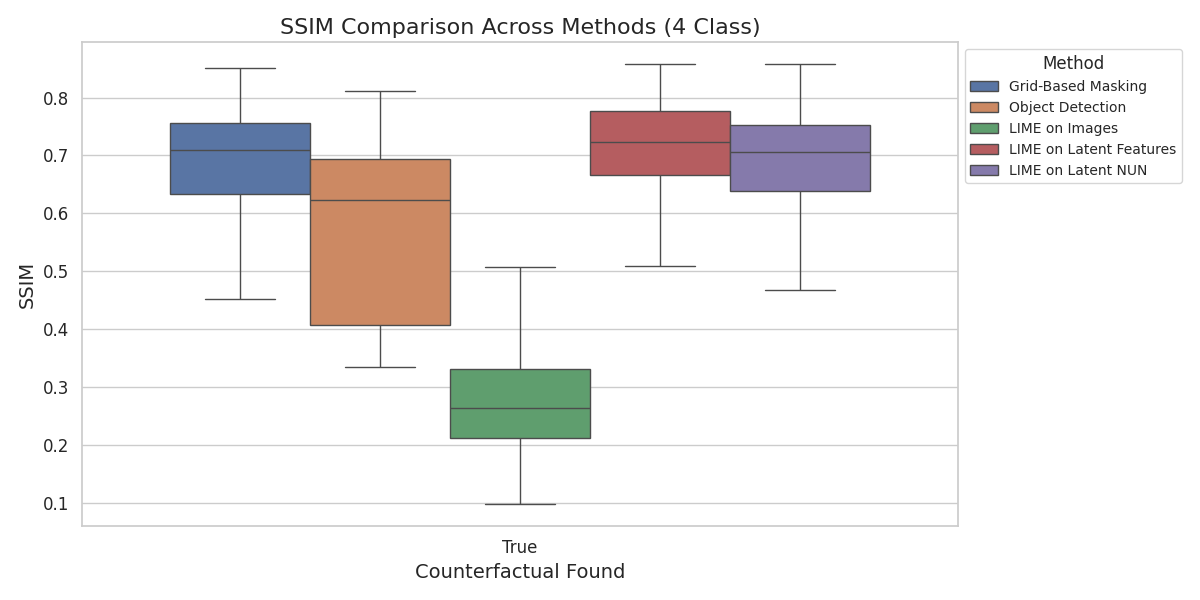
\includegraphics[width=\textwidth]{img/masking_results/ssim_boxplot_4_class.png}
    \caption{
        SSIM comparison across methods in the multi-class setting. SSIM values range from 0.0 to 1.0, where 1.0 indicates perfect structural similarity (images are visually identical in structure, contrast, and luminance), and 0.0 indicates no similarity. Higher SSIM values reflect more realistic and semantically faithful counterfactual reconstructions. Methods like latent feature space masking and Grid-Based masking generally achieve better perceptual quality.
    }
    \label{fig:ssim_boxplot}
\end{figure}

\begin{figure}[htbp]
    \centering
    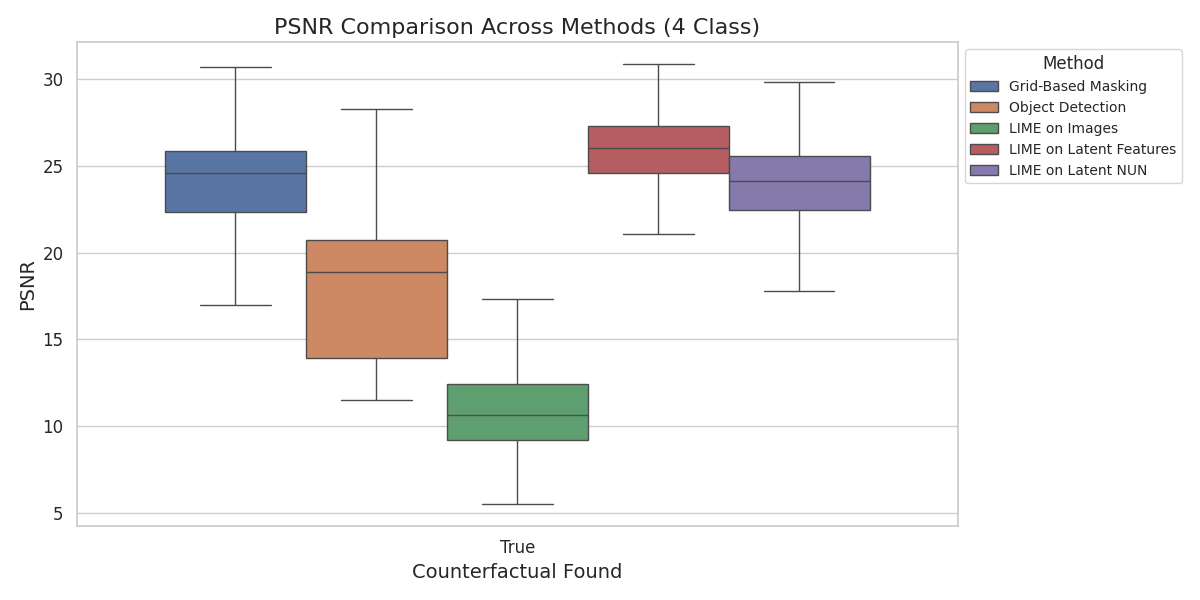
\includegraphics[width=0.85\textwidth]{img/masking_results/psnr_boxplot_4_class.png}
    \caption{
        PSNR comparison across methods in the 4-class setting. PSNR (Peak Signal-to-Noise Ratio) measures pixel-level similarity in decibels (dB). Higher values (typically above 25 dB) indicate sharper, less noisy reconstructions. Lower PSNR suggests significant deviation from the original image. Grid-Based and latent-space masking techniques yield the highest PSNR values, while image-space LIME results in noticeable quality loss.
    }
    \label{fig:psnr_boxplot}
\end{figure}


\vspace{1em}


\subsection{Efficiency: Time Complexity and Execution Time}
Although LIME on Latent NUN based masking produces high-quality explanations, it is the most computationally expensive, with a total runtime exceeding 263 minutes. In contrast, the Grid-Based method completes in just 13 minutes while still achieving competitive coverage and validity.



\subsection{Qualitative Examples of Counterfactual Explanations} \label{subsubsec:qualitative_examples}
To complement the quantitative evaluation of counterfactual explanation ussing different masking methods, qualitative visual analyses were conducted to assess the visual plausibility, semantic preservation, and discriminative alterations introduced by each masking technique. These visual examples help contextualize how each method perturbs the input to find counterfactual explanations that lead to prediction changes.

Individual counterfactual examples for all five masking methods Grid-Based Masking, Object Detection-Based Masking, LIME on Image, LIME on Latent Features, and LIME on Latent using NUN are provided in \cref{sec:feature_masking_pipeline} (see Figures~\ref{fig:grid_ce_example}--\ref{fig:object_detection_masking}). Each figure narratively presents:

\begin{itemize}
    \item The original input image and its predicted class,
    \item The type of masking applied (e.g., grid, object, latent),
    \item The reconstructed image after masking via the VAE,
    \item The change in prediction resulting from the perturbation.
\end{itemize}

This structure highlights the causally relevant regions identified by each method and their impact on the classification outcome.

Each method is qualitatively evaluated based on:
\begin{itemize}
    \item Semantic fidelity: Whether the essential image structure is preserved after masking and reconstruction.
    \item Visual realism: The plausibility of the counterfactual image.
    \item Effectiveness: Whether the counterfactual successfully changes the predicted class.
\end{itemize}

\vspace{0.5em}

To consolidate these comparisons, Table~\ref{tab:cf_visual_examples} provides an overview of one representative counterfactual explanation per method. These samples were selected from the test set where class flips occurred, illustrating how each masking technique alters the input to change the classifier's decision.

\begin{table}[htbp]
    \centering
    \caption{Representative counterfactual explanations across different masking methods. In the original images, the label is \textbf{STOP}; however, the counterfactual explanation shows \textbf{GO} due to the removal of the STOP sign.}
    \label{tab:cf_visual_examples}
    \begin{tabular}{>{\centering\arraybackslash}p{3.5cm} >{\centering\arraybackslash}c >{\centering\arraybackslash}c}
        \toprule
        \textbf{Masking Method} & \textbf{Original Image (STOP)} & \textbf{Counterfactual Explanation (GO)} \\
        \midrule
        Grid-Based Masking & 
        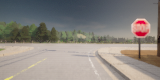
\includegraphics[width=0.3\textwidth]{img/masking_results/original.png} & 
        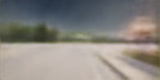
\includegraphics[width=0.3\textwidth]{img/masking_results/grid_cf.png} \\
        \addlinespace
        Object Detection Masking & 
        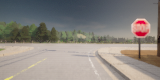
\includegraphics[width=0.3\textwidth]{img/masking_results/original.png} & 
        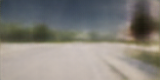
\includegraphics[width=0.3\textwidth]{img/masking_results/object_detection_cf.png} \\
        \addlinespace
        LIME on Image & 
        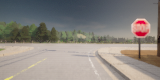
\includegraphics[width=0.3\textwidth]{img/masking_results/original.png} & 
        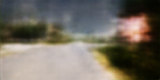
\includegraphics[width=0.3\textwidth]{img/masking_results/lime_image_cf.png} \\
        \addlinespace
        LIME on Latent & 
        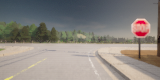
\includegraphics[width=0.3\textwidth]{img/masking_results/original.png} & 
        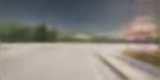
\includegraphics[width=0.3\textwidth]{img/masking_results/lime_latent_cf.png} \\
        \addlinespace
        LIME on Latent NUN & 
        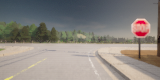
\includegraphics[width=0.3\textwidth]{img/masking_results/original.png} & 
        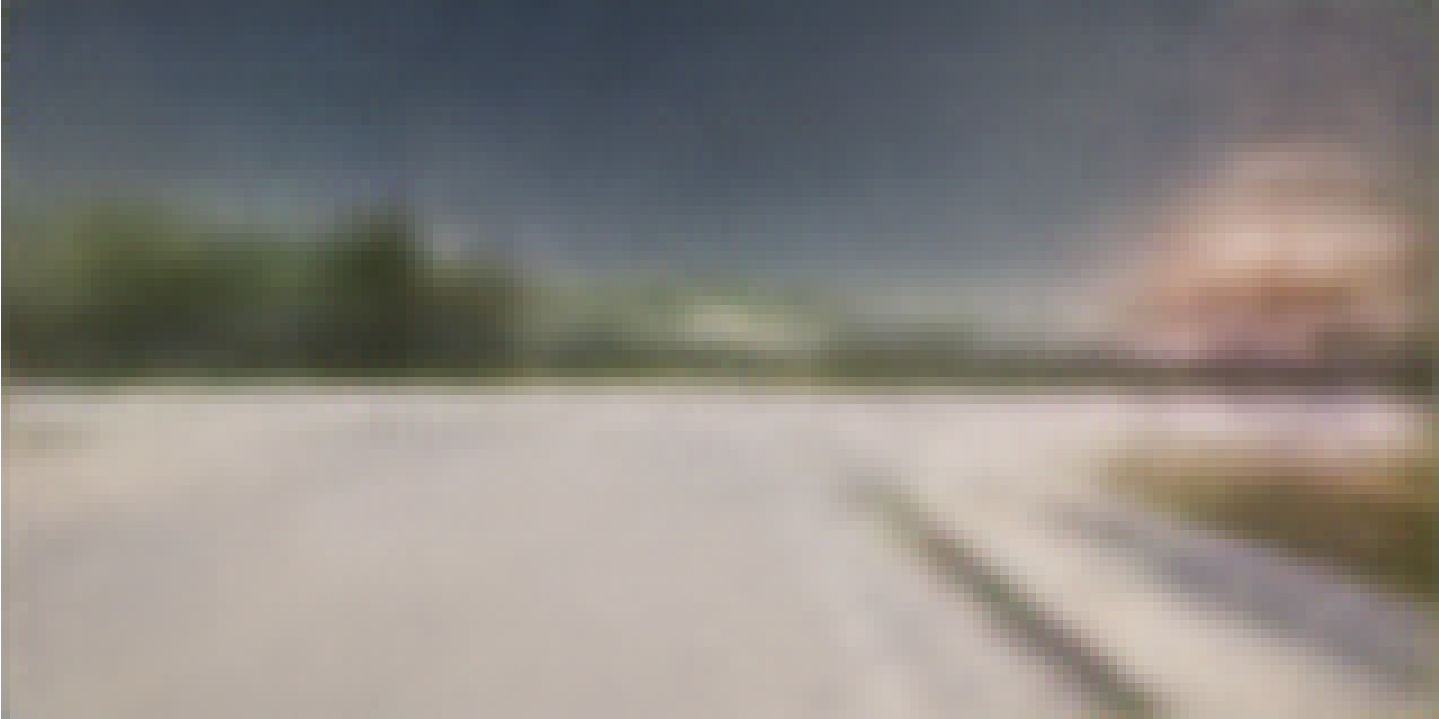
\includegraphics[width=0.3\textwidth]{img/masking_results/lime_NUN_cf.png} \\
        \bottomrule
    \end{tabular}
\end{table}

\textbf{Observations:}
\begin{itemize}
    \item \textbf{Grid-Based Masking:} Often introduces localized changes with some visible artifacts but successfully flips the class in most cases. It demonstrates good semantic targeting, although the visual naturalness may sometimes be compromised.
    \item \textbf{Object Detection Masking:} Attempts to remove salient objects. However, due to limitations in YOLOv5's detection performance on this dataset, many regions are missed. This leads to lower counterfactual success rates and less informative counterfactuals. Object detection masking is retained here primarily for completeness.
    \item \textbf{LIME on Image:} Produces counterfactuals that are visually intuitive by masking semantically important regions (e.g., road signs, motion cues). Although the reconstructions are perceptually realistic, the region selection can sometimes lack subtlety.
    \item \textbf{LIME on Latent:} Directly alters internal representations, often resulting in blurry or implausible reconstructions. This can lead to noisy or confusing counterfactuals that fail to reliably flip the class.
    \item \textbf{LIME on Latent NUN:} Achieves the best balance by minimally perturbing only the most relevant latent features. Its counterfactuals are both semantically meaningful and visually realistic, leading to successful class flips with minimal distortion.
\end{itemize}

\vspace{1em}

Together, these qualitative comparisons reinforce the quantitative results presented earlier (Figures~\ref{fig:bar_chart_ce_count_multi}--\ref{fig:venn_comparison}). In particular, LIME on Latent based masking using NUN method consistently generates the most faithful and effective counterfactual explanations. The visual clarity and semantic integrity of its outputs further confirm its practical utility for explainability in autonomous driving models.


\subsection{Discussions on Counterfactual Explanation Generation via
Masking Techniques}
The results demonstrates that:
\begin{itemize}
    \item LIME on Latent feature based masking using NUN method is the most effective method overall, generating high-quality, class-discriminative, and valid counterfactual explanations across all driving actions . But, computationally expensive.
    \item Grid-Based Masking provides a strong baseline with significantly lower computation time and excellent multi-class performance.
    \item LIME on Latent feature based masking is limited in both coverage and interpretability.
    \item Although LIME based masking on Images performs well in certain scenarios, its higher execution time and lower effectiveness for LEFT transitions reduce its appeal. For visual purpose these images are really distorted and added with more noise after reconstruction, the reason is because after the masking LIME covers most of the important region where it is masked the pixels with zero. The VAE is not trained on these kind of images the reconstrcutions are really bad.
    \item Objcet detection based masking on images performs very bad as YOLO v5 models fails to detect the objects in the dataset. This further failed in masking the objects which led to failure in the counterfatual explanantiosn generation. 
\end{itemize}
These results strongly support the adoption of latent-space counterfactual techniques particularly LIME on Latent feature based masking using NUN method for enhanced explainability in autonomous driving models.












\section{Overview of the Evaluation Strategy} \label{sec:human_evluation}

While traditional quantitative metrics such as SSIM and PSNR offer insight into the visual quality of reconstructed counterfactual images, they do not fully reflect human judgment regarding interpretability, plausibility, or realism. As noted by Delaney et al.~\cite{DELANEY2023103995}, counterfactual explanations are meant to fulfill human explanation goals and must therefore be evaluated with human-centered metrics. This is especially crucial in high-stakes domains such as autonomous driving, where explanations must not only be technically valid but also intuitively understandable and semantically coherent from a user's perspective.

To incorporate this human-centered evaluation, we developed a web-based application using FastAPI for backend processing and Jinja2 for rendering the frontend. The system was designed to present users with the original input image, its predicted label, and four corresponding counterfactual explanations—each generated using a different masking technique: Grid-Based Masking, LIME on Images, LIME on Latent Features, and LIME on Latent Features using the NUN method. To ensure fairness and avoid bias, the interface randomized the order of counterfactuals and concealed the identity of the underlying methods. Participants were only shown the prediction labels associated with each counterfactual image, not the technique used to generate it. A screenshot of the evaluation interface is provided in Appendix~\ref{app:web_interface}, Figure~\ref{fig:app:form_ui}.

Each user was asked to evaluate the counterfactual explanations based on three criteria: Interpretability (how clearly the image highlights the minimal change required to alter the model’s prediction), Plausibility (how realistic and contextually appropriate the modified image appears), and Visual Coherence (whether the transformation affects only necessary regions while preserving the rest of the scene). These aspects were rated on a Likert scale of 1 (poor) to 5 (excellent). Users also had the option to provide qualitative comments to elaborate on their assessments.

The system randomized the order of counterfactual images and concealed the identities of the masking methods, labeling each explanation only with its class prediction to reduce bias. The selected samples were those for which all four methods successfully generated counterfactuals—see Section~\ref{subsubsec:masking_method_overlap} for selection criteria.



\subsection{Quantitative Analysis of User Ratings} \label{subsubsec:quantitative_analysis_of_user_ratings}
To address RQ4 (Which counterfactual explanation method is preferred by users when selecting among generated explanations of the same original image, and what factors influence user preference?) we conducted an in-depth analysis of the collected human ratings. The anonymized evaluation labels were internally mapped to the respective methods Counterfactual\_1 corresponds to Grid-Based Masking, Counterfactual\_2 to LIME on Image Masking, Counterfactual\_3 to LIME on Latent Features, and Counterfactual\_4 to LIME on Latent Features using the NUN method.


The results of the user study, visualized in Figure~\ref{fig:bar_plot_user_eval}, indicate that LIME on Latent Features using NUN (Method 4) consistently achieved the highest average ratings across all three evaluation criteria. Grid-Based Masking (Method 1) emerged as the second-most preferred technique, also scoring well on all aspects. In contrast, LIME on Image Masking (Method 2) received the lowest ratings, with participants frequently citing issues like over-masking, loss of visual detail, and unrealistic reconstructions. LIME on Latent Features without NUN (Method 3) performed moderately, offering acceptable quality but lacking the precision of NUN-based selection.

\begin{figure}[htbp]
    \centering
    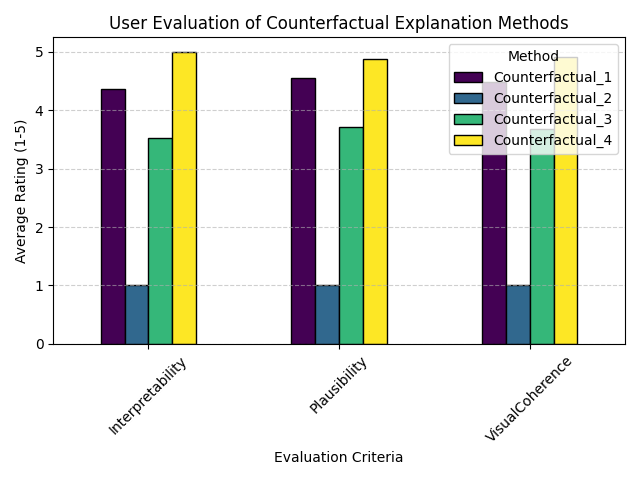
\includegraphics[width=0.75\textwidth]{img/human_rating_results/bar_plot_user_evaluations.png}
    \caption{Average user ratings (scale 1–5) for each counterfactual method across all evaluation criteria.}
    \label{fig:bar_plot_user_eval}
\end{figure}

To provide a consolidated view, we generated a heatmap (Figure~\ref{fig:heatmap_user_eval}) summarizing the average user ratings per method for each evaluation criterion. This visual representation further confirms the overall superiority of Method 4, which maintained high scores with minimal variance across interpretability, plausibility, and visual coherence.

Further breakdowns by criterion are presented in Figures~\ref{fig:cf_interpretability}, \ref{fig:cf_plausibility}, and \ref{fig:cf_visualcoherence}. These plots show that Method 4 achieved near-perfect ratings (~5) in all categories. In particular, its strength in visual coherence demonstrates its ability to isolate semantically meaningful edits without disrupting background consistency. Grid-Based Masking also scored high in interpretability and coherence, making it a reliable and efficient alternative, especially where computational speed is important. In contrast, Method 2 struggled across all dimensions, reflecting limitations in the VAE’s capacity to reconstruct images with zero-masked regions introduced by LIME on Image masking.

\begin{figure}[htbp]
    \centering
    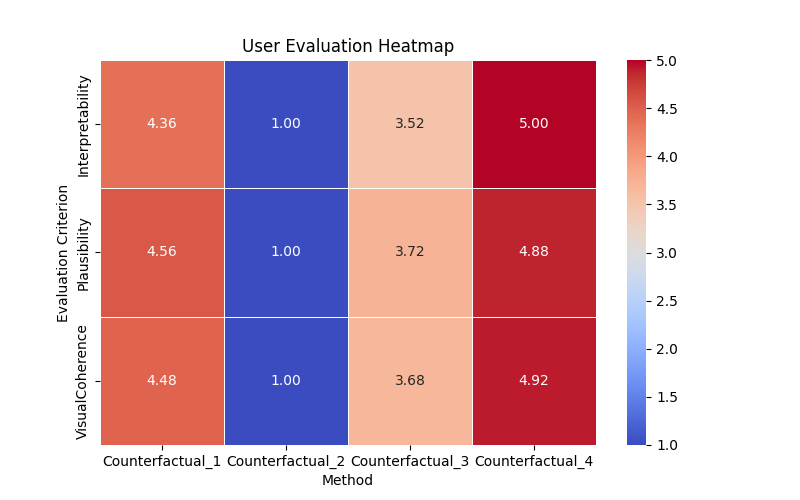
\includegraphics[width=0.6\textwidth]{img/human_rating_results/heatmap_user_evaluations.png}
    \caption{Heatmap of average user ratings for each counterfactual method and evaluation criterion.}
    \label{fig:heatmap_user_eval}
\end{figure}

\vspace{0.5em}
\paragraph{Per-Criterion Analysis.}
Figures~\ref{fig:cf_interpretability}--\ref{fig:cf_visualcoherence} present a breakdown of average ratings per evaluation criterion:

\begin{itemize}
    \item \textbf{Interpretability:} LIME on Latent NUN (Method 4) was rated highest (~5), followed by Grid-Based Masking. LIME on Image received the lowest ratings due to aggressive masking of salient regions.
    \item \textbf{Plausibility:} Again, Method 4 led the ratings, reflecting its ability to produce realistic modifications. Grid-Based Masking served as a strong secondary option, while Method 2 lagged due to unconvincing reconstructions.
    \item \textbf{Visual Coherence:} Method 4 stood out by preserving contextual elements and background consistency, especially when minimal edits sufficed for counterfactual generation.
\end{itemize}

\begin{figure}[h]
    \centering
    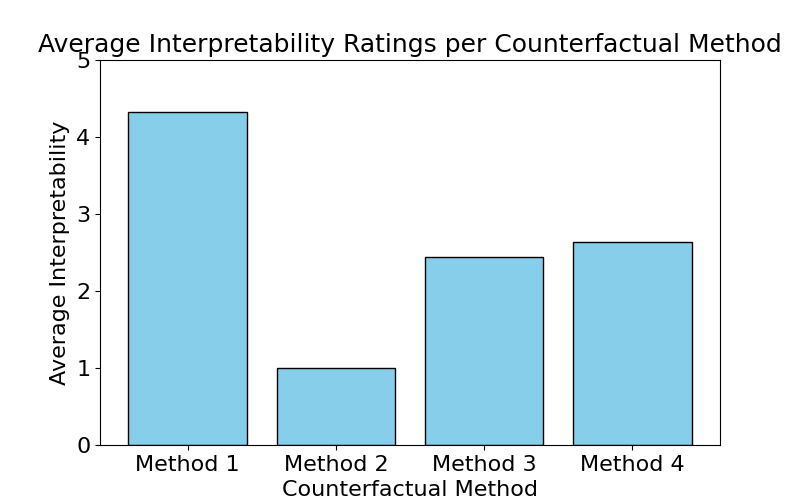
\includegraphics[width=0.5\textwidth]{img/human_rating_results/Interpretability_ratings.png}
    \caption{Average interpretability ratings per counterfactual method.}
    \label{fig:cf_interpretability}
\end{figure}

\begin{figure}[h]
    \centering
    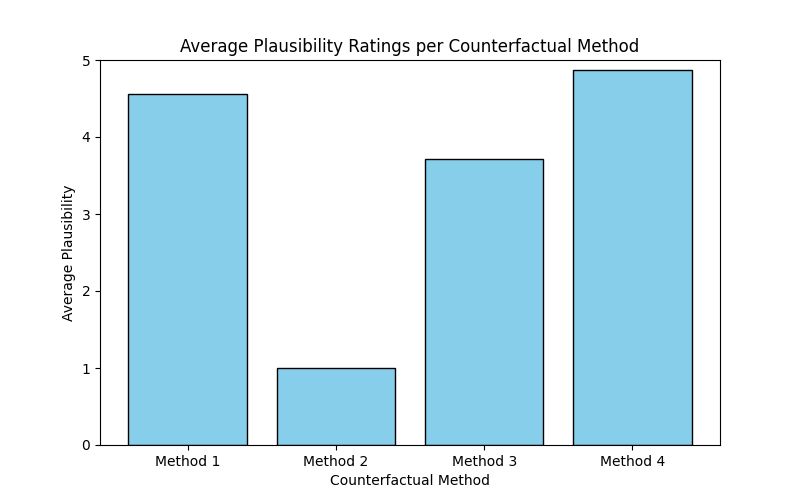
\includegraphics[width=0.5\textwidth]{img/human_rating_results/Plausibility_ratings.png}
    \caption{Average plausibility ratings per counterfactual method.}
    \label{fig:cf_plausibility}
\end{figure}

\begin{figure}[h]
    \centering
    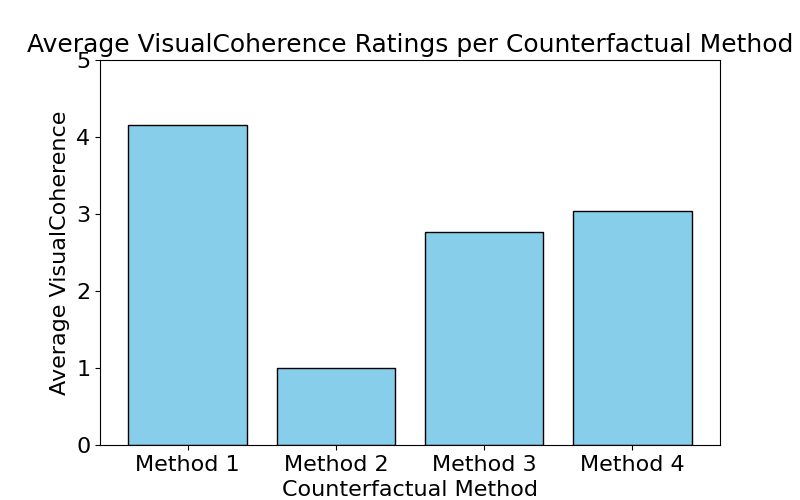
\includegraphics[width=0.5\textwidth]{img/human_rating_results/VisualCoherence_ratings.png}
    \caption{Average visual coherence ratings per counterfactual method.}
    \label{fig:cf_visualcoherence}
\end{figure}

\vspace{0.5em}
\subsection{Qualitative Feedback and Discussion}
Participant comments provided additional depth to the numerical ratings. Explanations generated via LIME on Latent NUN were frequently described as “realistic,” “semantically consistent,” and “preserving important details.” Users appreciated the minimal yet impactful changes these counterfactual explanations found, allowing for intuitive understanding of model decisions. Grid-Based Masking was praised for producing “clean,” “structured,” and “easily interpretable” edits. On the other hand, LIME based masking on Latent Features received mixed feedback, while some edits were described as “acceptable,” others were criticized for being blurry or poorly localized. Most negative feedback was associated with LIME on Image Masking, where participants described counterfactual explanations found images as “dark,” “unrecognizable,” or “lacking detail,” highlighting a significant gap in visual realism.

These results underscore the importance of human-centric validation in explainable AI systems. While algorithmic evaluations such as counterfactual explanation coverage (interpreted as validity in our work), SSIM, and PSNR provide essential performance benchmarks, they often fail to capture the nuances of human perception. In real-world deployments particularly in safety-critical domains like autonomous driving interpretability must align with human intuition to foster trust and acceptance. Our findings demonstrate that the LIME on Latent features masking using NUN method and Grid based masking method consistently outperforms other approaches across both quantitative metrics and user-based assessments, making it the most effective strategy for generating counterfactual explanations that are both technically sound and intuitively meaningful.

By narrowing the gap between human expectations and algorithmic reasoning, such methods offer a promising path toward building more trustworthy AI systems. While this study represents a significant step in aligning model explanations with user understanding, further advancements are necessary to achieve deeper trust. Enhancing generative models, refining latent manipulations, and incorporating more expressive human feedback mechanisms could further bridge the trust gap, bringing us closer to AI systems that behave not only accurately but also transparently and collaboratively.